\chapter{Funzioni}
% =============================================================================

\section{Funzioni astratte}

\defn{Funzione}{
Siano $A, B \ne \emptyset$. Si chiama \textbf{funzione} $f: A \rarr B$ una legge che associa \textbf{ad ogni elemento di $A$ uno ed un solo elemento di $B$}.
Si può anche scrivere:
\[
f: x \in A \mapsto y = f(x) \in B
\]
dove $y$ è l'\textbf{immagine} di $x$ mediante $f$.
}

\begin{itemize}
    \item $A$ si dice \textbf{dominio} di $f$ (insieme di esistenza)
    \item $B$ si dice \textbf{codominio} di $f$
    \item L'insieme
    \[
    f(A) = \{\, y \in B \mid \exists x \in A : y = f(x) \,\}
    \]
    si chiama \textbf{immagine} di $A$
    \item Sia $y \in B$, con $f^{-1}(y)$ indichiamo il seguente insieme:
    \[
    f^{-1}(y) = \{\, x \in A \mid f(x) = y \,\}
    \]
    Questo insieme può avere, a seconda dei casi, nessuno ($\emptyset$), uno o più elementi.
    \item L'insieme
    \[
    G(f) = \{\, (x, f(x)) \mid x \in A \,\}
    \]
    si chiama \textbf{grafico} di $f$
\end{itemize}

\subsection{Restrizione}

\defn{Restrizione}{
Sia $f: A \rarr B$ con $A, B \ne \emptyset$.
Sia $E \subseteq A$, $E \ne \emptyset$.
La funzione
\[
g: E \rarr B, \quad g(x) = f(x) \text{ per ogni } x \in E
\]
si chiama \textbf{restrizione di $f$ su $E$} e si indica con $f|_E$.
}

\subsection{Funzioni composte}
Siano $A, B, C \ne \emptyset$ e siano $f: A \to B$ e $g: B \to C$.
Allora si definisce la \textbf{funzione composta} $g \circ f: A \to C$ mediante
\[
(g \circ f)(x) = g(f(x)), \quad \forall x \in A
\]
dove $(g \circ f)(x)$ è l'immagine di $x$ tramite la composizione di $f$ e $g$.

\ex{
\[
f(x) = x + 1, \quad f: \mathbb{R} \to \mathbb{R} \\
g(x) = x^3, \quad g: \mathbb{R} \to \mathbb{R}
\]
Allora:
\[
(g \circ f)(x) = g(f(x)) = (x + 1)^3, \quad x \in \mathbb{R} \\
(f \circ g)(x) = f(g(x)) = x^3 + 1, \quad x \in \mathbb{R}
\]
Questi esempi mostrano chiaramente che la composizione \textbf{non è commutativa}.
}

\subsection{Funzioni suriettive}
Una funzione $f: A \to B$ si dice \textbf{suriettiva} se l'immagine coincide con il codominio, cioè:
\[
\forall b \in B, \ \exists a \in A \mid f(a) = b
\]
In una funzione suriettiva la controimmagine di ogni elemento del codominio \textbf{non può essere vuota}.

\subsection{Funzioni iniettive}
Una funzione $f: A \to B$ si dice \textbf{iniettiva} se elementi distinti del dominio hanno immagini distinte, cioè:
\[
\forall x_1, x_2 \in A, \ f(x_1) = f(x_2) \implies x_1 = x_2
\]
oppure equivalentemente:
\[
x_1, x_2 \in A, \ x_1 \ne x_2 \implies f(x_1) \ne f(x_2)
\]
In una funzione iniettiva la controimmagine di ogni elemento del codominio può avere \textbf{al massimo un elemento}.

\subsection{Funzioni biettive}
Una funzione $f: A \to B$ si dice \textbf{biettiva} se è sia iniettiva che suriettiva.
\begin{itemize}
    \item Esiste quindi una \textbf{corrispondenza biunivoca} tra gli elementi del dominio e del codominio.
    \item La controimmagine di ogni elemento del codominio possiede \textbf{esattamente un elemento}.
    \item In simboli:
    \[
    f(A) = B, \quad x_1 \ne x_2 \implies f(x_1) \ne f(x_2)
    \]
\end{itemize}

\subsection{Identità}
\defn{Funzione Identità}{
Sia $A \ne \emptyset$.
La \textbf{funzione identità} su $A$, indicata con $i_A$, è definita da:
\[
i_A: x \in A \mapsto x \in A
\]
}

Se la funzione è biettiva si definisce la funzione inversa
\[
f^{-1}: B \to A, \quad y \in B \mapsto x = f^{-1}(y)
\]
Avendo $f: A \to B$ e $f^{-1}: B \to A$ possiamo comporle per ottenere le funzioni identità di $A$ e identità di $B$ ($i_A$ e $i_B$):
\begin{itemize}
    \item $f \circ f^{-1}: y \in B \mapsto y \in B = i_B$
    \item $f^{-1} \circ f: x \in A \mapsto x \in A = i_A$
\end{itemize}

Una funzione biettiva è anche \textbf{invertibile}, cioè esiste $f^{-1}: B \to A$ tale che:
\[
f^{-1}(f(x)) = x, \quad \forall x \in A
\]

L'esistenza della funzione inversa è ciò che ci permette di risolvere le disequazioni, prendiamo ad esempio la disequazione $x^2 \leq 8$:
\begin{itemize}
    \item La funzione potenza $f(x) = x^2$ non è invertibile su tutto $\mathbb{R}$, ma diventa invertibile se ristretta al dominio $\mathbb{R}^+_0$ (numeri reali non negativi). La sua inversa è la funzione radice quadrata $f^{-1}(y) = \sqrt{y}$, definita per $y \geq 0$.

    \item Utilizzando la funzione inversa, possiamo risolvere la disequazione $x^2 \leq 8$ applicando la radice quadrata a entrambi i membri. Tuttavia, dobbiamo considerare che $x^2$ è definita per tutti gli $x \in \mathbb{R}$, quindi dobbiamo separare i casi in base al segno di $x$:
    \begin{itemize}
        \item Se $x \geq 0$, allora $x = \sqrt{x^2} \leq \sqrt{8} = 2\sqrt{2}$.
        \item Se $x \leq 0$, allora $x = -\sqrt{x^2} \geq -\sqrt{8} = -2\sqrt{2}$.
    \end{itemize}

    \item Combinando i due casi, otteniamo la soluzione finale:
    \[
    -2\sqrt{2} \leq x \leq 2\sqrt{2}.
    \]
    Questo significa che tutti i valori di $x$ compresi tra $-2\sqrt{2}$ e $2\sqrt{2}$ soddisfano la disequazione $x^2 \leq 8$.
  \end{itemize}

\section{Funzioni Numeriche}
\subsection{Proprietà delle funzioni numeriche}
\subsubsection{Grafico della Funzione}

\defn{Grafico}{
Sia $f : A \subseteq \mathbb{R} \to \mathbb{R}$, con $A \neq \emptyset$.
Si chiama \emph{grafico} di $f$ l'insieme
\[
G(f) = \{(x, f(x)) \mid x \in A\} \subseteq \mathbb{R}^2.
\]
}

Nel piano cartesiano non esiste una relazione d'ordine.
Ad ogni funzione corrisponde un grafico.

\begin{figure}[h]
    \centering
    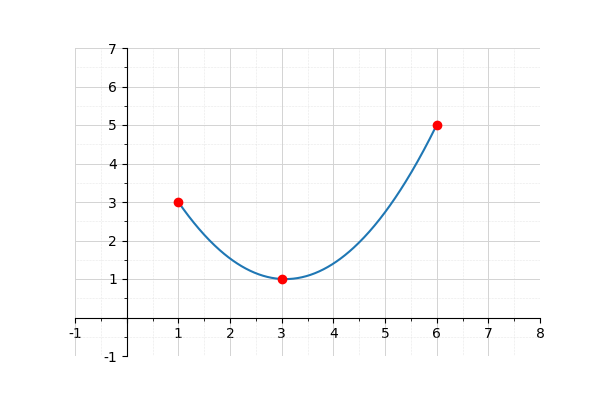
\includegraphics[width=0.7\textwidth]{./img/grafico.png} % sostituire con il file corretto
    \caption{Grafico della funzione}
    \label{fig:grafico_della_funzione}
  \end{figure}
  
Dal grafico di una funzione possiamo ricavare informazioni come il dominio e il codominio anche senza conoscere la legge precisa:
\[
A = [1, 6], \quad f(A) = B = [1, 5].
\]

Dal grafico possiamo capire anche se la funzione è iniettiva.

\subsubsection{Funzione Inversa}

Una funzione è invertibile se e solo se, fissato un valore $y$, esiste una sola $x$ tale che $f(x) = y$.

Se la funzione è invertibile, il grafico della sua inversa è
\[
G(f^{-1}) = \{(y, f^{-1}(y)) \mid y \in f(A)\}.
\]

\begin{figure}[h]
    \centering
    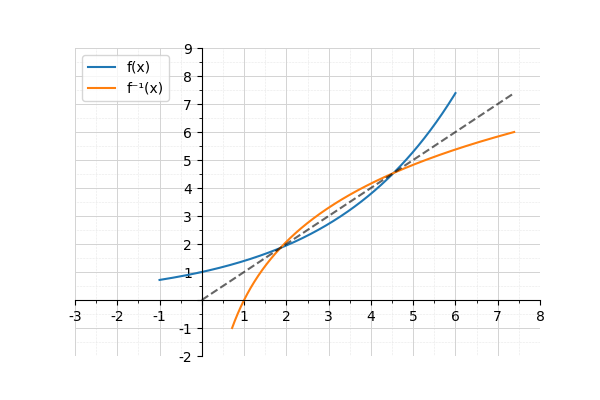
\includegraphics[width=0.7\textwidth]{./img/funzione_inversa.png} % sostituire con il file corretto
    \caption{Grafico della funzione inversa}
    \label{fig:funzione_inversa}
\end{figure}

\subsection{Funzioni Pari e Dispari}

\defn{Proprietà di simmetria}{
  Sia $f: \mathbb{R} \to \mathbb{R}$.  
  La funzione $f$ si dice \emph{pari} se
  \[
    f(-x) = f(x), \quad \forall x \in \mathbb{R},
  \]
  cioè se ha simmetria rispetto all'asse $y$.  

  La funzione $f$ si dice \emph{dispari} se
  \[
    f(-x) = -f(x), \quad \forall x \in \mathbb{R}.
  \]

  La funzione $f$ si dice \emph{periodica} di periodo $t \in \mathbb{R}$ se
  \[
    f(x) = f(x+t), \quad \forall x \in \mathbb{R}.
  \]
}

\begin{figure}[h]
    \centering
    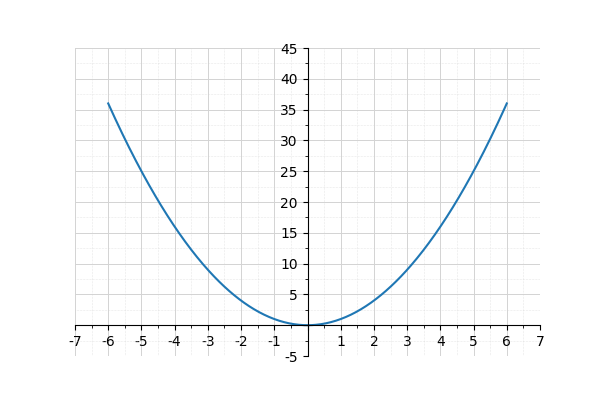
\includegraphics[width=0.7\textwidth]{./img/funzione_pari.png}
    \caption{Esempio di funzione pari}
    \label{fig:funzione_pari}
\end{figure}

\begin{figure}[h]
    \centering
    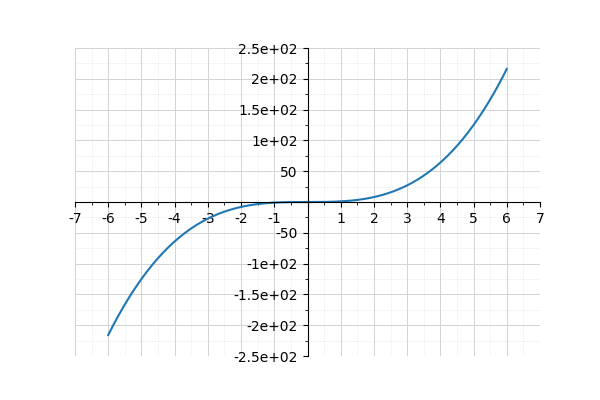
\includegraphics[width=0.7\textwidth]{./img/funzione_dispari.png}
    \caption{Esempio di funzione dispari}
    \label{fig:funzione_dispari}
\end{figure}

\begin{figure}[h]
    \centering
    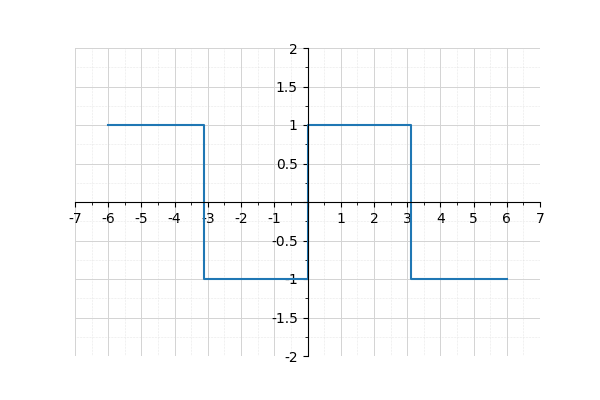
\includegraphics[width=0.7\textwidth]{./img/funzione_periodica.png}
    \caption{Esempio di funzione periodica}
    \label{fig:funzione_periodica}
\end{figure}

\subsection{Funzioni Limitate}

\defn{Funzione superiormente limitata}{
  Sia $f: A \subseteq \mathbb{R} \to \mathbb{R}$ con $A \neq \emptyset$.  
  La funzione $f$ si dice \emph{superiormente limitata} se $f(A)$ è superiormente limitata, cioè se
  \[
    \exists K \in \mathbb{R} \text{ tale che } f(x) \leq K, \quad \forall x \in A.
  \]
}

\defn{Funzione inferiormente limitata}{
  La funzione $f$ si dice \emph{inferiormente limitata} se $f(A)$ è inferiormente limitata, cioè se
  \[
    \exists c \in \mathbb{R} \text{ tale che } c \leq f(x), \quad \forall x \in A.
  \]
}

\defn{Funzione limitata}{
  La funzione $f$ si dice \emph{limitata} se è sia inferiormente che superiormente limitata, cioè se
  \[
    \exists c, K \in \mathbb{R} \text{ tali che } c \leq f(x) \leq K, \quad \forall x \in A.
  \]
}

\defn{Estremo superiore}{
  Si definisce \emph{estremo superiore} di $f(A)$ e si indica con $\sup f(A)$.
}

\defn{Estremo inferiore}{
  Si definisce \emph{estremo inferiore} di $f(A)$ e si indica con $\inf f(A)$.
}

\subsection{Massimo e Minimo}

\defn{Massimo}{
  Sia $f: A \subseteq \mathbb{R} \to \mathbb{R}$ con $A \neq \emptyset$.  
  Se $f(A)$ ha un massimo $M$, diremo che $f$ ha un massimo e scriveremo
  \[
    M = \max f(A).
  \]
  Essendo $M \in f(A)$, esiste $x_M \in A$ tale che $f(x_M) = M$, che si chiama \emph{punto di massimo}. Il punto di massimo non è necessariamente unico.
}

\begin{figure}[h]
    \centering
    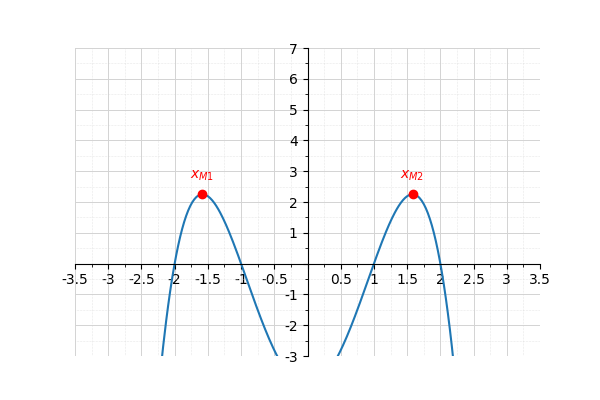
\includegraphics[width=0.7\textwidth]{./img/massimi_della_funzione.png}
    \caption{Esempio di funzione con due punti di massimo}
    \label{fig:punto_di_massimo}
\end{figure}

\defn{Minimo}{
  Se $f(A)$ ha un minimo $m$, diremo che $f$ ha un minimo e i punti $x_m \in A$ tali che $f(x_m) = m$ si chiamano \emph{punti di minimo}.
}

\subsection{Funzioni Monotone}

\defn{Monotona crescente}{
  Sia $f: A \subseteq \mathbb{R} \to \mathbb{R}$ con $A \neq \emptyset$.  
  La funzione $f$ si dice \emph{monotona crescente} se
  \[
    x_1 < x_2, \ x_1, x_2 \in A \implies f(x_1) \leq f(x_2),
  \]
  e \emph{strettamente monotona crescente} se
  \[
    x_1 < x_2 \implies f(x_1) < f(x_2).
  \]
}

\begin{figure}[h]
    \centering
    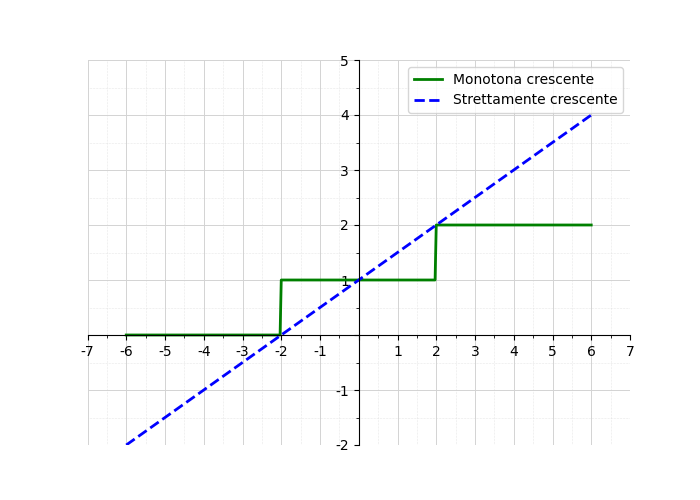
\includegraphics[width=0.7\textwidth]{./img/monotone_crescenti.png}
    \caption{Esempio di funzioni crescenti}
    \label{fig:funzione_crescente}
\end{figure}

\defn{Monotona decrescente}{
  La funzione $f$ si dice \emph{monotona decrescente} se
  \[
    x_1 < x_2 \implies f(x_1) \geq f(x_2),
  \]
  e \emph{strettamente monotona decrescente} se
  \[
    x_1 < x_2 \implies f(x_1) > f(x_2).
  \]
}

\begin{figure}[h]
    \centering
    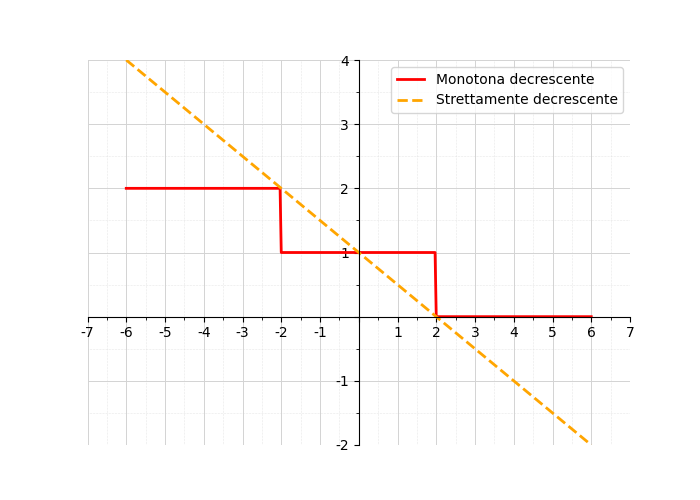
\includegraphics[width=0.7\textwidth]{./img/monotone_decrescenti.png}
    \caption{Esempio di funzioni decrescenti}
    \label{fig:funzione_decrescente}
\end{figure}

Inoltre valgono le seguenti proprietà:
\begin{itemize}
  \item Una funzione strettamente monotona è iniettiva.
  \item Se $f$ è invertibile e monotona, anche $f^{-1}$ è monotona della stessa tipologia.
\end{itemize}

\section{Funzioni Elementari}
\subsection{Funzioni lineari (o affini)}

Sia 
\[
f(x) = a x + b, \quad a, b \in \mathbb{R}, \quad a \neq 0.
\]

\begin{figure}[h]
    \centering
    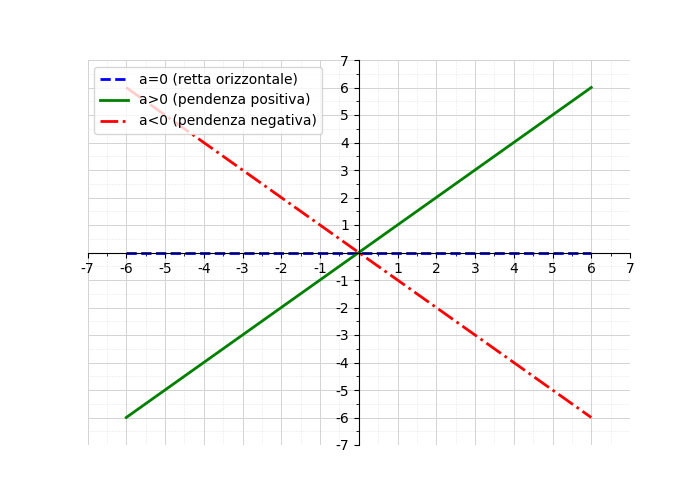
\includegraphics[width=0.7\textwidth]{./img/lineari_combinato.png}
    \caption{Grafico della funzione lineare}
    \label{fig:funzione_lineare}
\end{figure}

Proprietà della funzione lineare:
\begin{itemize}
    \item Se $a > 0$, la funzione è crescente.
    \item Se $a < 0$, la funzione è decrescente.
    \item Se $f(x) = x$ o $f(x) = -x$, la funzione coincide con una bisettrice.
\end{itemize}

\subsection{Funzione valore assoluto}

Sia
\[
|x| = 
\begin{cases} 
x, & \text{se } x \ge 0, \\
-x, & \text{se } x < 0,
\end{cases}
\quad x \in \mathbb{R}, \quad |x| : \mathbb{R} \to [0, +\infty).
\]

\begin{figure}[h]
    \centering
    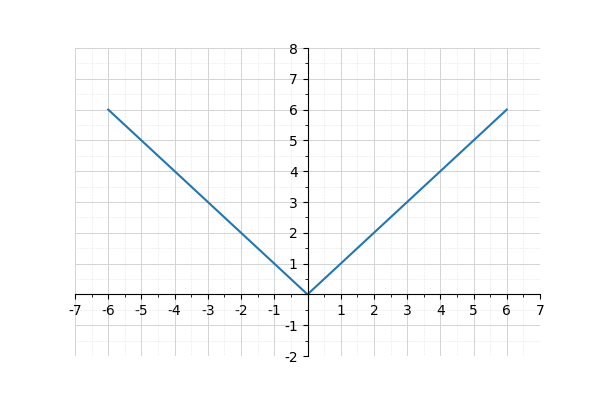
\includegraphics[width=0.7\textwidth]{./img/funzione_valore_assoluto.png}
    \caption{Grafico della funzione valore assoluto}
    \label{fig:funzione_valore_assoluto}
\end{figure}


  

Proprietà della funzione valore assoluto:
\begin{enumerate}
    \item $|x| \ge 0$ per ogni $x \in \mathbb{R}$.
    \item $|x| = 0 \iff x = 0$.
    \item $|-x| = |x|$, quindi la funzione è pari.
    \item $|x_1 \cdot x_2| = |x_1| \cdot |x_2|$.
    \item $|x| \le a \iff -a \le x \le a$.
    \item $|x| \ge a \iff x \le -a \ \text{o} \ x \ge a$.
    \item Per ogni $x_1, x_2 \in \mathbb{R}$ vale la \emph{disuguaglianza triangolare}:
    \[
    |x_1 + x_2| \le |x_1| + |x_2|.
    \]
    Dimostrazione:
    \begin{align*}
    -|x_1| \le x_1 \le |x_1|, \quad -|x_2| \le x_2 \le |x_2| \\
    \implies -(|x_1| + |x_2|) \le x_1 + x_2 \le |x_1| + |x_2| \\
    \implies |x_1 + x_2| \le |x_1| + |x_2|.
    \end{align*}
  \end{enumerate}
\subsection{Funzione potenza (con esponente in $\mathbb{N}$)}

Sia
\[
f: x \in \mathbb{R} \mapsto x^n
\]
Allora:
\begin{itemize}
  \item $f(x) \in [0, +\infty)$ per $n$ pari
  \item $f(x) \in \mathbb{R}$ per $n$ dispari
\end{itemize}

La funzione è quindi:
\[
f(x) = x^n
\]

\subsubsection{Caso $n$ pari}
\begin{figure}[H]
    \centering
    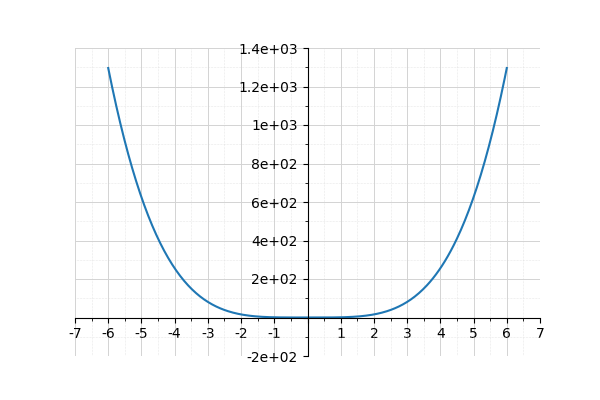
\includegraphics[width=0.7\textwidth]{./img/esponente_pari.png}
    \caption{Grafico della funzione potenza per $n$ pari}
    \label{fig:esponente_pari}
\end{figure}
\FloatBarrier{}

\begin{itemize}
  \item La funzione è pari
  \item $x^n \geq 0 \quad \forall x \in \mathbb{R}$, e $x^n = 0 \iff x = 0$
  \item Non è globalmente monotona:
  \begin{itemize}
    \item $x^n$ è strettamente crescente per $x \geq 0$
    \item $x^n$ è strettamente decrescente per $x \leq 0$
  \end{itemize}
  \item $\displaystyle \sup_{x \in \mathbb{R}} x^n = +\infty$
  \item $\displaystyle \inf_{x \in \mathbb{R}} x^n = \min_{x \in \mathbb{R}} x^n = 0$
\end{itemize}


\subsubsection{Caso $n$ dispari}

\begin{figure}[H]
    \centering
    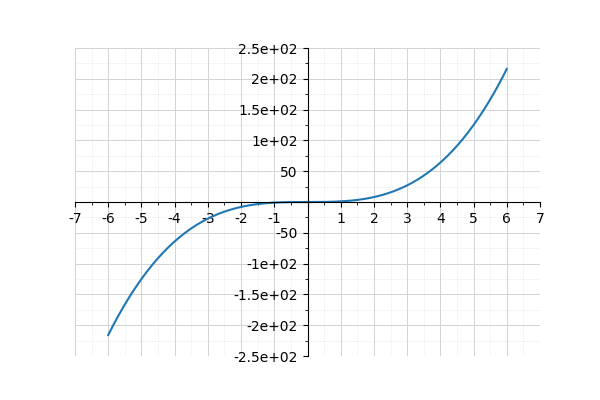
\includegraphics[width=0.7\textwidth]{./img/esponente_dispari.png}
    \caption{Grafico della funzione per $n$ dispari}
    \label{fig:esponente_dispari}
\end{figure}
\FloatBarrier
  
\begin{itemize}
\item La funzione è dispari
\item La funzione è strettamente monotona crescente (quindi è iniettiva $\implies$ invertibile)
\item $\inf_{x \in \mathbb{R}} x^n = -\infty$
\item $\sup_{x \in \mathbb{R}} x^n = +\infty$
\end{itemize}

\subsubsection{Proprietà comuni}
Proprietà valide per entrambi i casi:
\begin{itemize}
\item $x^{n_1} \cdot x^{n_2} = x^{n_1+n_2} \quad \forall x \in \mathbb{R}, \forall n_1, n_2 \in \mathbb{N}$
\item $\frac{x^{n_1}}{x^{n_2}} = x^{n_1-n_2} \quad \text{se } x \neq 0 \text{ e } n_1 \geq n_2$
\item $(x^{n_1})^{n_2} = x^{n_1 \cdot n_2} \quad \forall x \in \mathbb{R}, \forall n_1, n_2 \in \mathbb{N}$
\item $(x \cdot y)^n = x^n \cdot y^n \quad \forall x, y \in \mathbb{R}, \forall n \in \mathbb{N}$
\item $|x^n| = |x|^n \quad \forall x \in \mathbb{R}, \forall n \in \mathbb{N}$
\end{itemize}



\subsubsection{Funzione potenza con esponente negativo}
\defn{Potenza inversa}{
  Si definisce $x^{-n}$ (con $x \neq 0$) come $x^{-n} := \frac{1}{x^n}$
  Poniamo $x^0 = 1$ se $x \neq 0$. A questo punto abbiamo definito la funzione $x^n$ con $n \in \mathbb{Z}$.
}

La funzione potenza con $n$ negativo è definita in:
\begin{itemize}
\item $\mathbb{R} \setminus \{0\}$ per $n$ dispari
\item $(0, +\infty)$ per $n$ pari
\end{itemize}

Grafico della funzione $f(x) = x^n$ con $n$ negativo pari:
\begin{figure}[H]
    \centering
    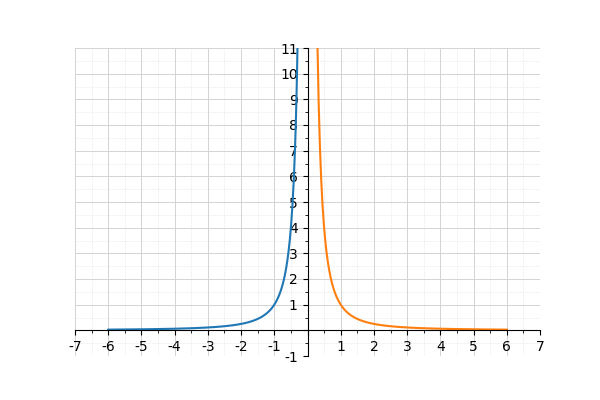
\includegraphics[width=0.7\textwidth]{./img/esponente_neg_pari.png}
    \caption{Grafico della funzione per $n$ negativo pari}
    \label{fig:esponente_neg_pari}
\end{figure}
\FloatBarrier

Grafico della funzione $f(x) = x^n$ con $n$ negativo dispari:
\begin{figure}[H]
    \centering
    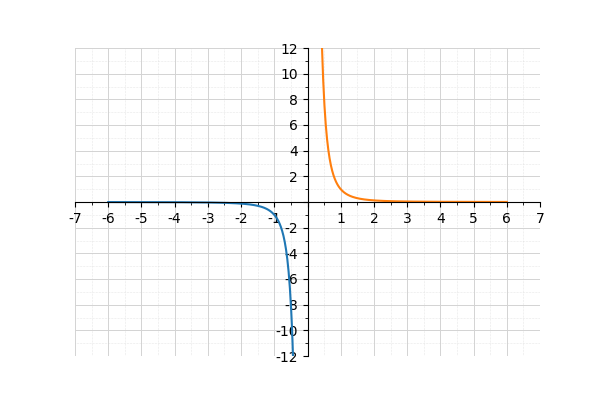
\includegraphics[width=0.7\textwidth]{./img/esponente_neg_dispari.png}
    \caption{Grafico della funzione per $n$ negativo dispari}
    \label{fig:esponente_neg_dispari}
\end{figure}
\FloatBarrier

\subsubsection{Funzione potenza con esponente reale}

La funzione potenza con esponente reale è definita come:
\[
x^\alpha : \; ]0, +\infty[ \; \longmapsto \; ]0, +\infty[, \quad \alpha \in \mathbb{R}
\]

e può essere espressa come:
\[
x^\alpha = e^{\alpha \ln x}
\]

A seconda del valore di $\alpha$, la funzione presenta diversi comportamenti:

\begin{itemize}
\item Se $\alpha > 1$, la funzione è **strettamente crescente** e **convessa**.
\item Se $0 < \alpha < 1$, la funzione è **strettamente crescente** e **concava**.
\item Se $\alpha < 0$, la funzione è **strettamente decrescente**.
\end{itemize}

\begin{figure}[H]
    \centering
    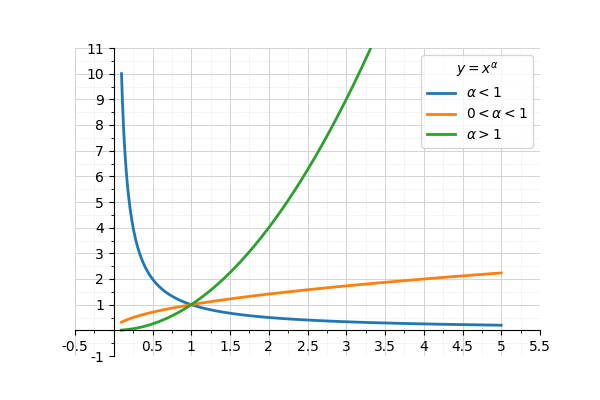
\includegraphics[width=0.7\textwidth]{./img/potenze_reali.png}
    \caption{Grafico della funzione $x^\alpha$ per diversi valori di $\alpha$: $-1$, $0.5$, e $2$.}
    \label{fig:potenze_reali}
\end{figure}
\FloatBarrier

Nel caso di $\alpha$ positivo e frazionario (ad esempio $\alpha = \frac{1}{2}$), il dominio può essere esteso anche a $x = 0$, ossia $[0, +\infty[$.


\subsection{Funzione radice $n$-esima}

\subsubsection{Con esponente dispari}
La funzione potenza con esponente dispari è dotata di inversa: la radice $n$-esima.
$$\sqrt[n]{x}: \mathbb{R} \mapsto \mathbb{R} \quad \text{inversa di } x^n$$

\begin{figure}[H]
    \centering
    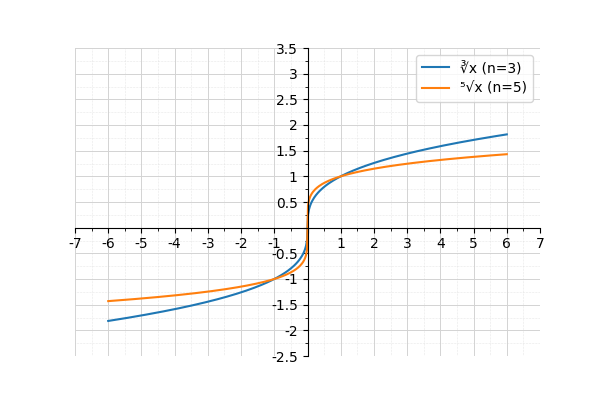
\includegraphics[width=0.7\textwidth]{./img/radice_dispari.png}
    \caption{Grafico della funzione radice $n$-esima con $n$ dispari}
    \label{fig:radice_dispari}
\end{figure}
\FloatBarrier

Proprietà:
\begin{itemize}
\item È strettamente crescente
\item È dispari
\item $\sqrt[n]{x^n} = x \quad \forall x \in \mathbb{R}$
\item $(\sqrt[n]{x})^n = x \quad \forall x \in \mathbb{R}$
\end{itemize}

\subsubsection{Con esponente pari}
La funzione potenza con esponente pari non è globalmente invertibile. Non la possiamo invertire in tutto $\mathbb{R}$; ci serve ridurre il dominio alla parte della funzione strettamente monotona crescente:
$$x^n|_{[0, +\infty[}: [0,+\infty[ \mapsto [0, +\infty[ $$

\begin{figure}[H]
    \centering
    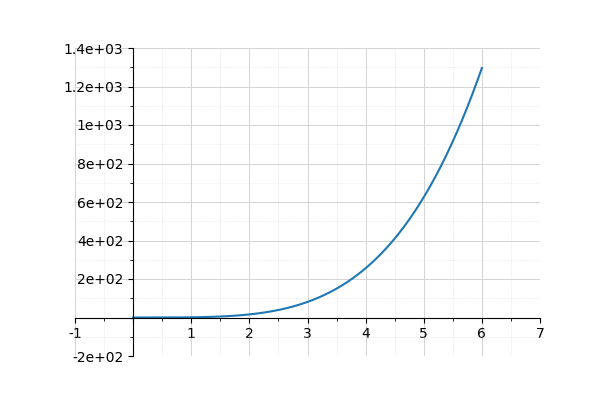
\includegraphics[width=0.7\textwidth]{./img/esponente_pari_ristretta.png}
    \caption{Grafico della restrizione della funzione potenza con $n$ pari}
    \label{fig:potenza_pari_ristretta}
\end{figure}
\FloatBarrier

La funzione inversa della restrizione è la radice $n$-esima:
$$\sqrt[n]{x}: [0, +\infty[ \mapsto [0, +\infty[ $$

\begin{figure}[H]
    \centering
    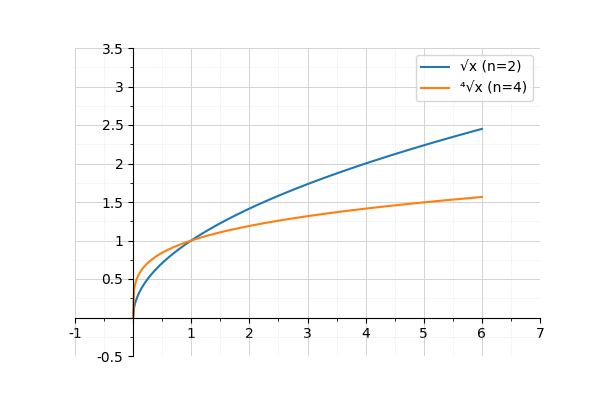
\includegraphics[width=0.7\textwidth]{./img/radice_pari.png}
    \caption{Grafico della funzione radice $n$-esima con $n$ pari}
    \label{fig:radice_pari}
\end{figure}
\FloatBarrier

Come cambiano le relazioni tra la funzione potenza e la sua inversa:
\begin{itemize}
\item $\sqrt[n]{x^n} = |x| \quad \forall x \in \mathbb{R}$
\item $(\sqrt[n]{x})^n = x \quad \forall x \geq 0$
\end{itemize}

\subsubsection{Proprietà comuni}
Proprietà valide per entrambi i casi:
\begin{itemize}
\item $\sqrt[n]{x} \cdot \sqrt[n]{y} = \sqrt[n]{x \cdot y}$ (con $x, y \geq 0$ per $n$ pari)
\item $x < y \implies \sqrt[n]{x} < \sqrt[n]{y}$ (con $x, y \geq 0$ per $n$ pari)
\item $\sqrt[n]{\sqrt[m]{x}} = \sqrt[n \cdot m]{x}$ (con $x \geq 0$ per $n$ o $m$ pari)
\item $\sqrt[n]{x^m} = x^{m/n}$ con $x \geq 0$, $m, n > 0$
\end{itemize}

\subsection{Funzione esponenziale}

Sia
\[
  a > 0, \quad a \neq 1, \quad a \in \mathbb{R}
\]
la base di una funzione esponenziale del tipo
\[
  f(x) = a^x \quad \text{con} \quad x \in \mathbb{R}, \; f(x) \in (0, +\infty)
\]

Per $a > 1$ si ha $a^b > 0 \quad \forall b \in \mathbb{R}$

Per $0 < a < 1$ si ha $a^b = \left(\frac{1}{a}\right)^b \quad \forall b \in \mathbb{R}$

\begin{figure}[H]
  \centering
  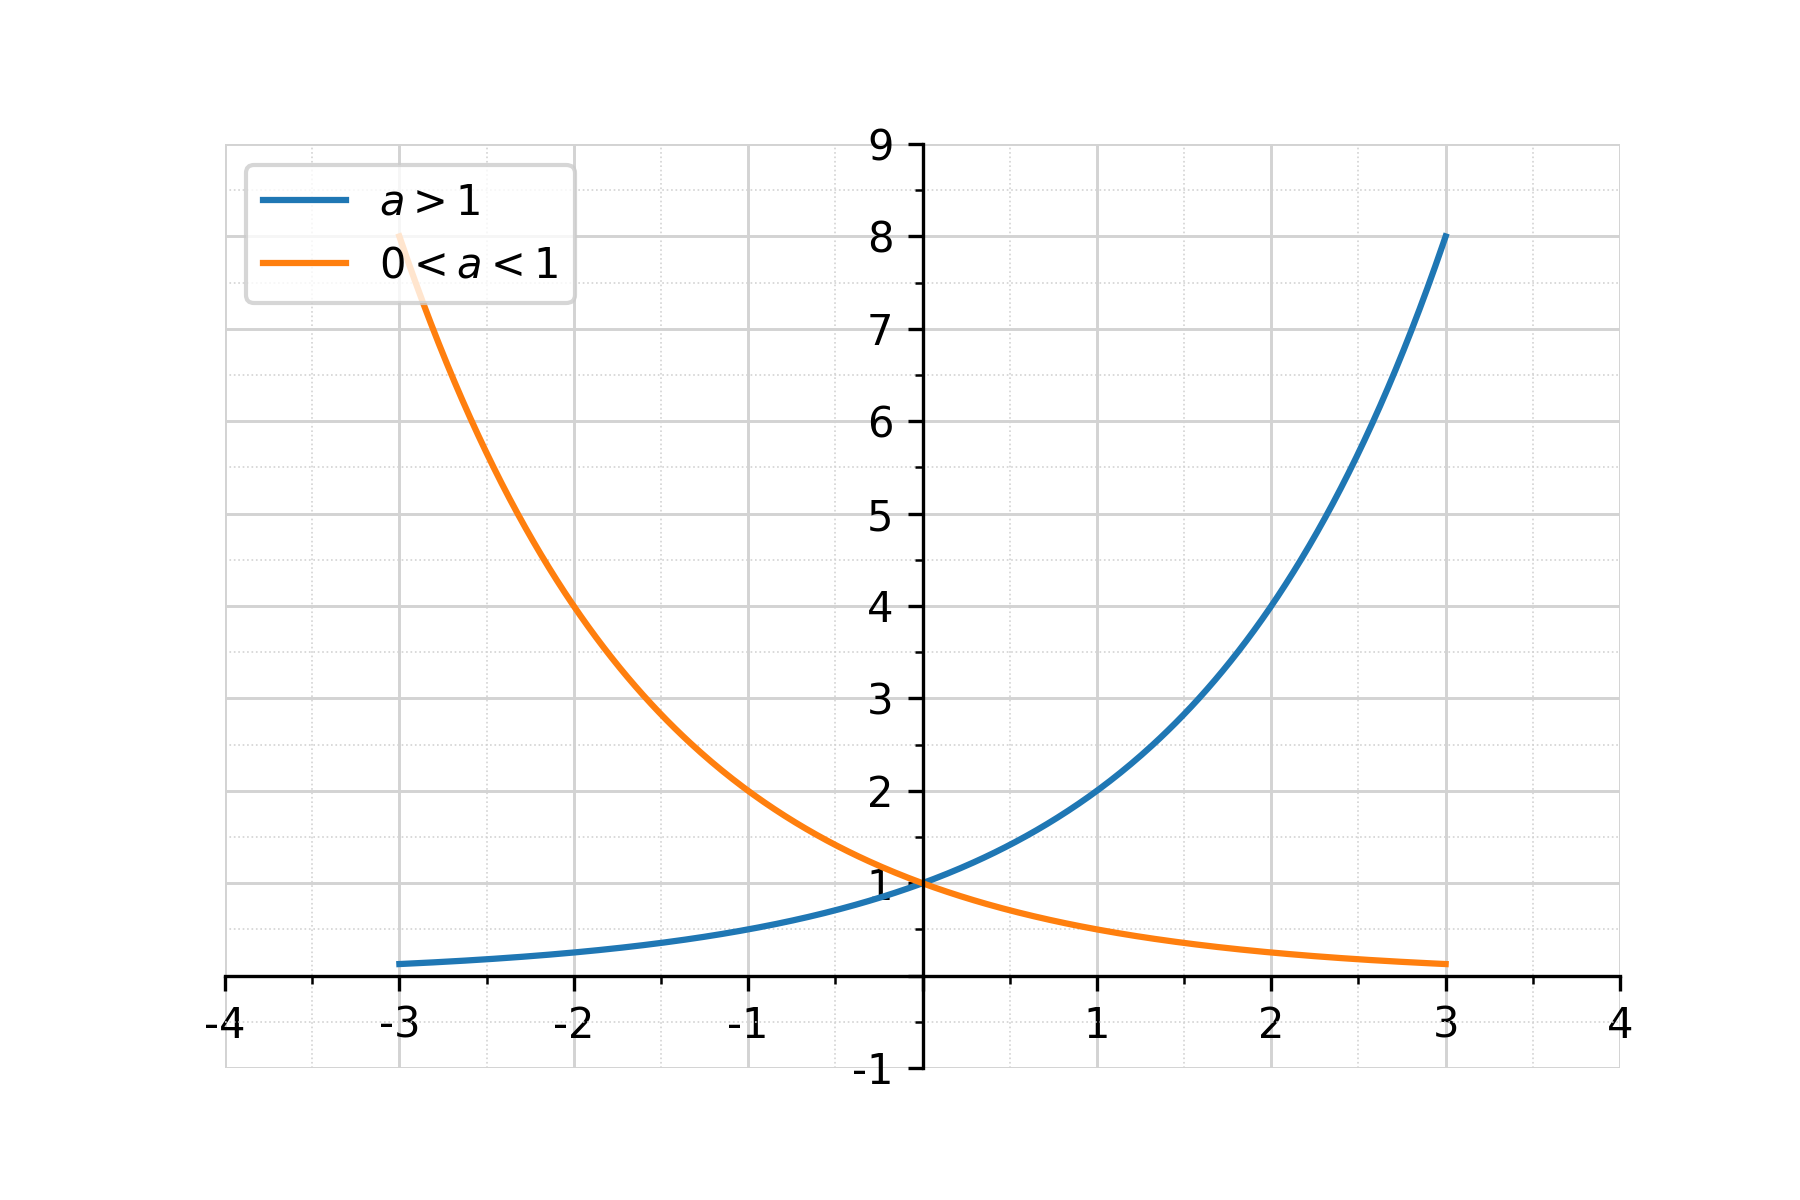
\includegraphics[width=0.7\textwidth]{./img/esponenziale.png}
  \caption{Grafico della funzione esponenziale per $a>1$ e $0<a<1$}
  \label{fig:funzione_esponenziale}
\end{figure}
\FloatBarrier

Proprietà della funzione esponenziale:
\begin{itemize}
  \item Se $a > 1$, la funzione è strettamente crescente.
  \item Se $0 < a < 1$, la funzione è strettamente decrescente.
  \item $a^x > 0 \quad \forall x \in \mathbb{R}$.
  \item $a^0 = 1$.
  \item $a^x \cdot a^y = a^{x + y}$.
  \item $(a^x)^y = a^{x \cdot y}$.
\end{itemize}


\subsection{Funzione Logaritmica}

La funzione logaritmica è l'inversa della funzione esponenziale $a^x$ con $a > 0$ e $a \neq 1$:
\[
  \log_a(x): ]0, +\infty[ \mapsto \R
\]

$a$ prende il nome di \textit{base del logaritmo},  
$x$ prende il nome di \textit{argomento del logaritmo}.

\begin{figure}[H]
  \centering
  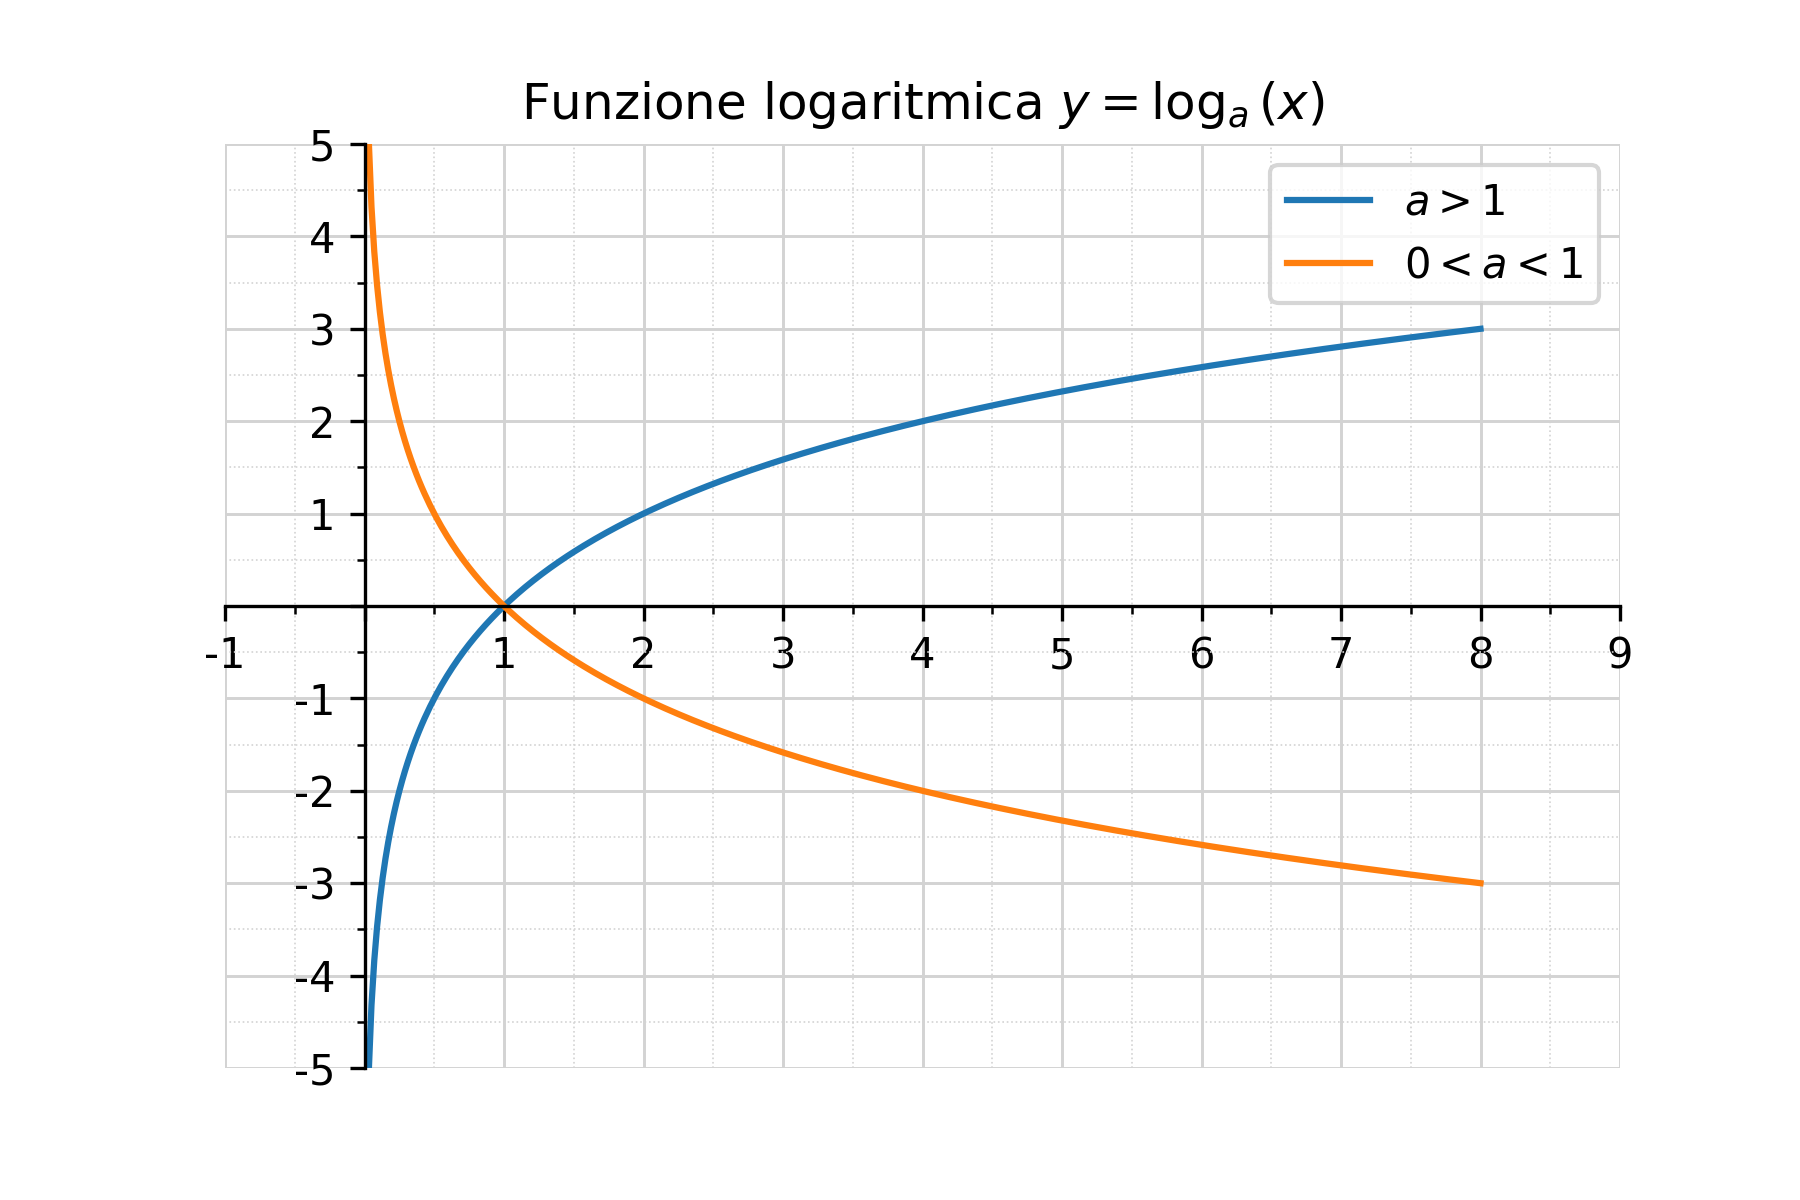
\includegraphics[width=0.7\textwidth]{./img/logaritmica.png}
  \caption{Grafico della funzione logaritmica per $a>1$ e $0<a<1$}
  \label{fig:funzione_logaritmica}
\end{figure}
\FloatBarrier

Relazioni di passaggio tra funzione esponenziale e logaritmica:
\[
\left\{
\begin{array}{l}
a^{\log_a(x)} = x \\
\log_a(a^x) = x \quad \forall x \in \R
\end{array}
\right.
\]

Proprietà dei logaritmi:
\begin{itemize}
  \item $\log_a(x \cdot y) = \log_a(x) + \log_a(y)$
  \item $\log_a\!\left(\dfrac{x}{y}\right) = \log_a(x) - \log_a(y)$
  \item $\log_a(x^{\alpha}) = \alpha \cdot \log_a(x)$
  \item $\log_a(x) = \dfrac{\log_b(x)}{\log_b(a)} \quad \forall b > 0, \; b \neq 1$
  \end{itemize}

  \section{Funzioni Trigonometriche Elementari}
Le funzioni trigonometriche sono funzioni di un angolo. Per definirle rigorosamente, si introduce il \textbf{radiante} come unità di misura e si utilizza la \textbf{circonferenza goniometrica}, ovvero una circonferenza di raggio unitario centrata nell'origine degli assi.

\begin{figure}[H]
    \centering
    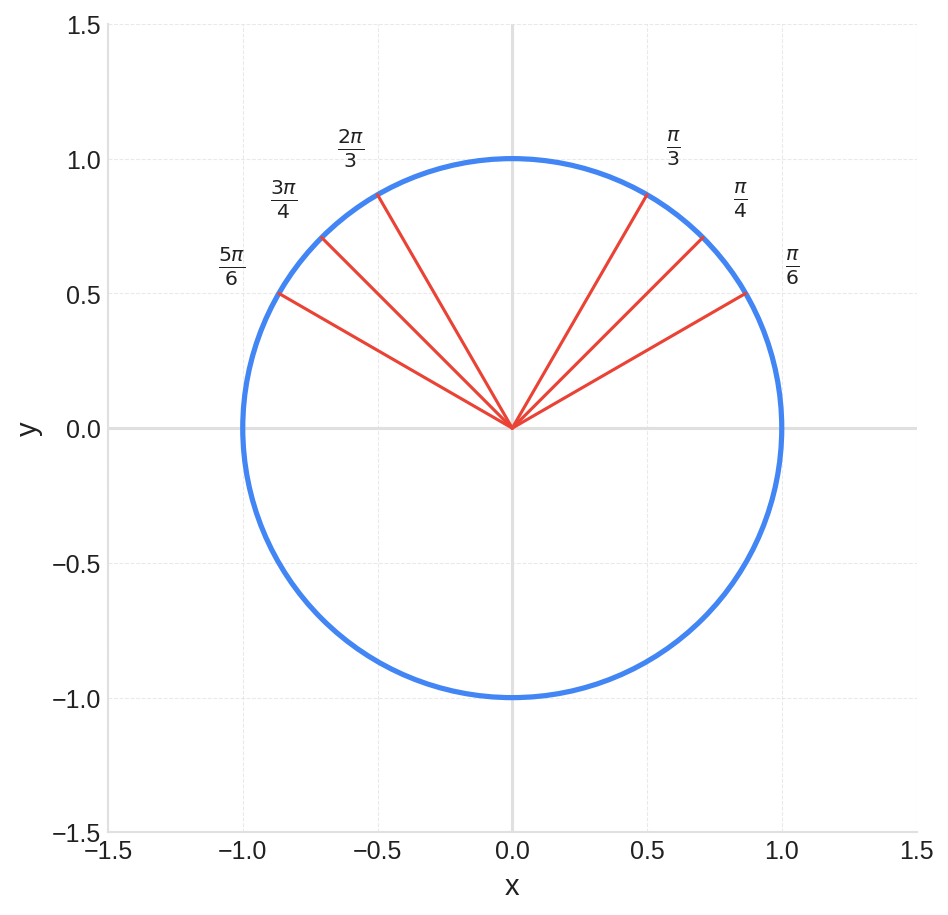
\includegraphics[width=0.5\textwidth]{./img/circonferenza_goniometrica.png}
    \caption{Circonferenza goniometrica con angoli notevoli.}
    \label{fig:circonferenza_goniometrica}
\end{figure}
\FloatBarrier

Dato un angolo \(\alpha\) in radianti, si identifica un punto \(P(x_p, y_p)\) sulla circonferenza. Dato che gli angoli in radianti sono adimensionali, posso ore definire fuzioni reali: le funzioni seno e coseno sono definite come le coordinate di questo punto.


\subsection{Funzioni Seno e Coseno}
\defn{Seno e Coseno}{
    Dato un punto \(P(x_p, y_p)\) sulla circonferenza goniometrica associato a un angolo \(\alpha\), si definisce:
    \begin{itemize}
        \item \textbf{Coseno:} \( \cos(\alpha) = x_p \) (ascissa di P)
        \item \textbf{Seno:} \( \sin(\alpha) = y_p \) (ordinata di P)
    \end{itemize}
}

\begin{figure}[H]
    \centering
    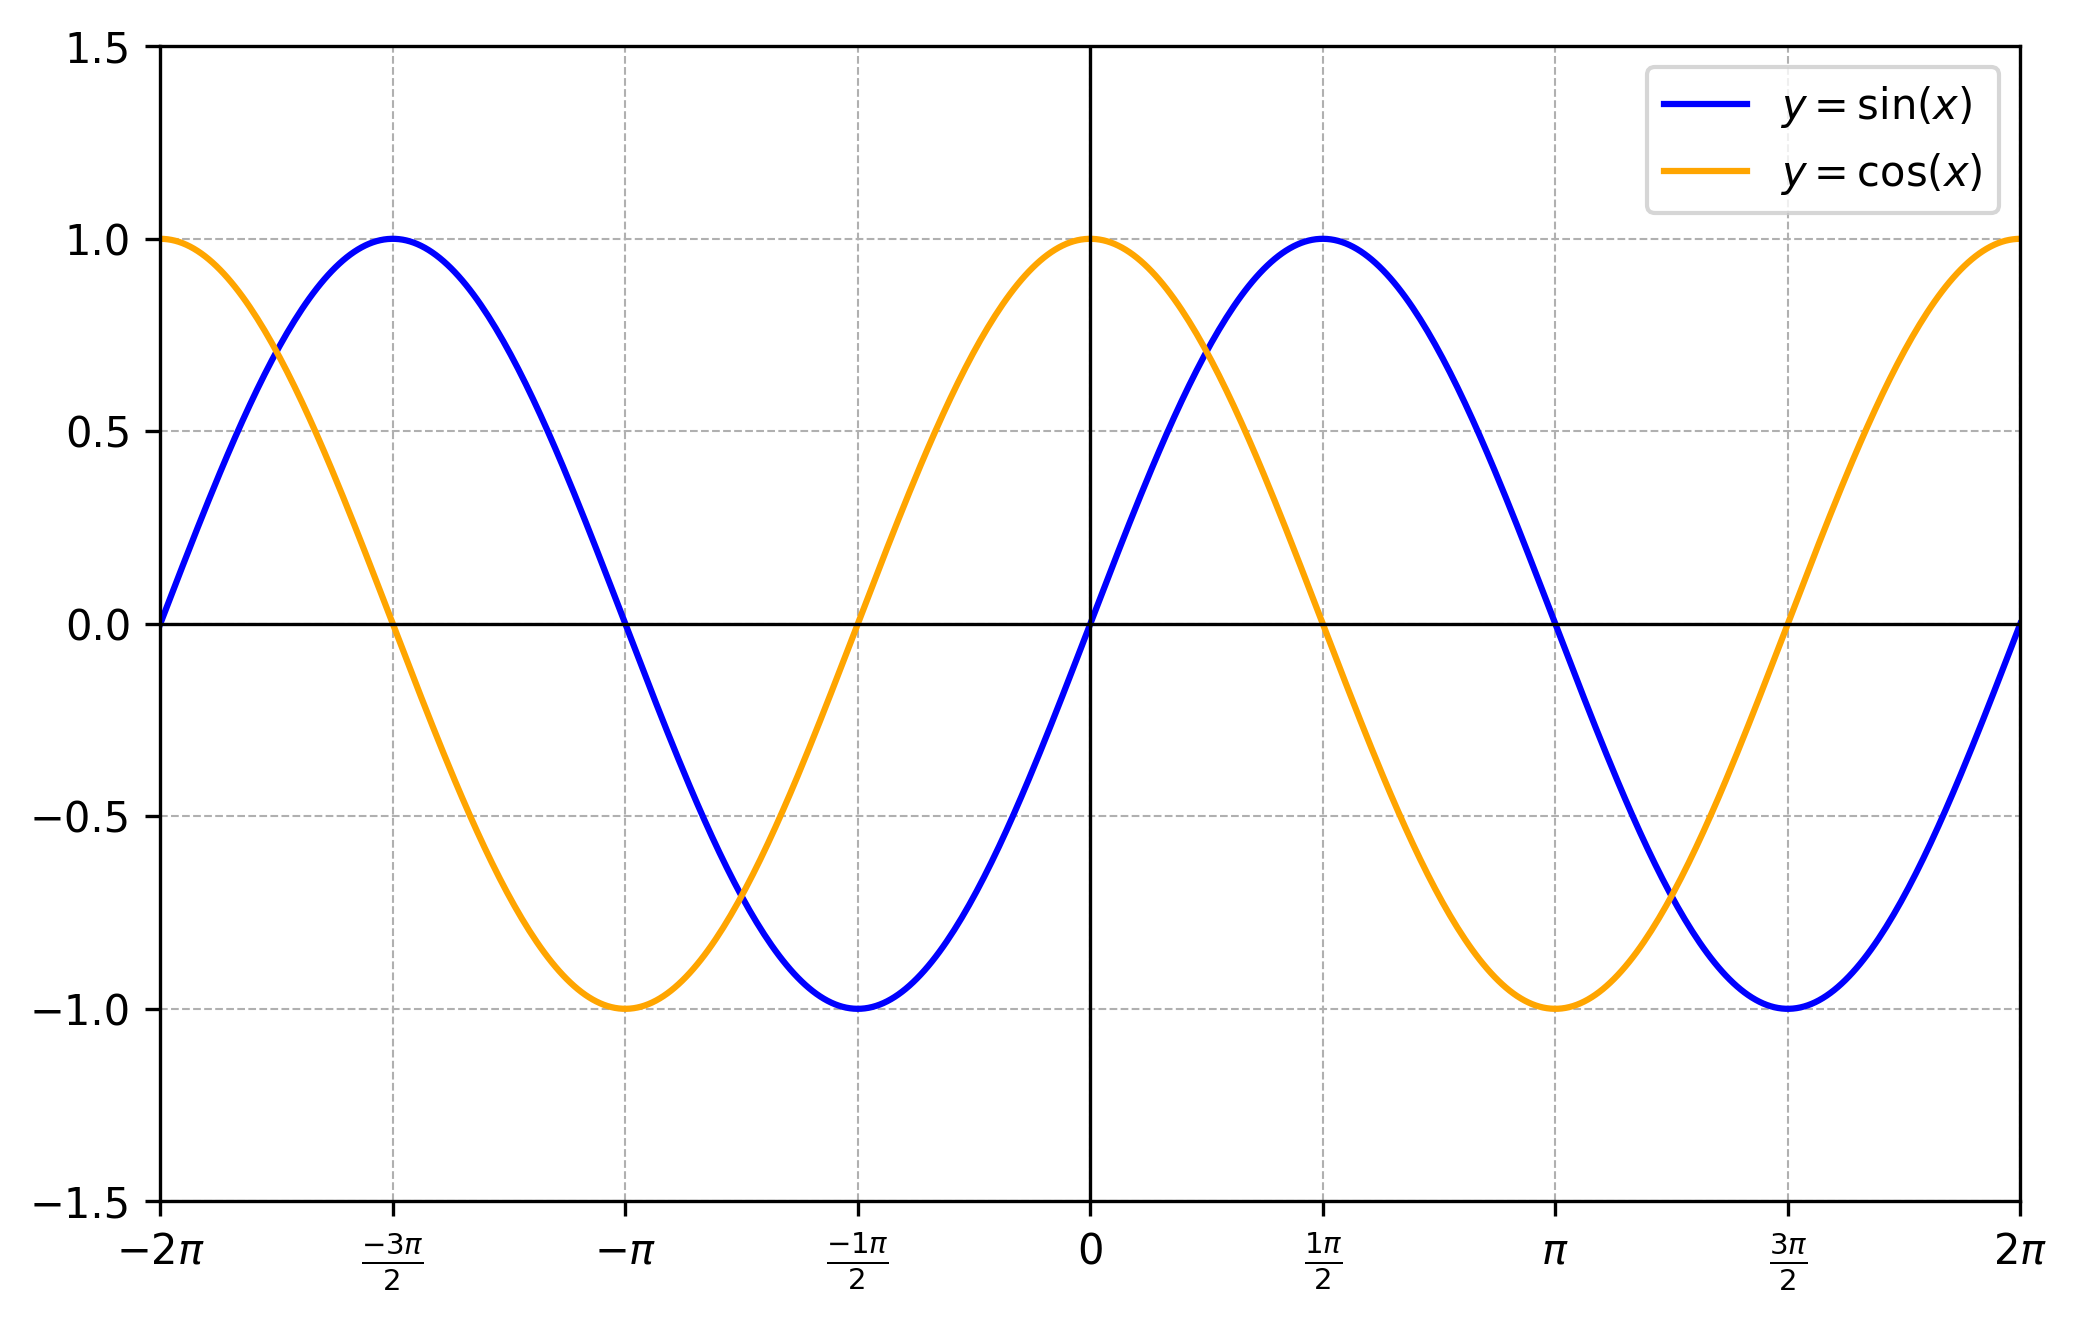
\includegraphics[width=0.8\textwidth]{./img/seno_coseno_grafici.png}
    \caption{Grafici delle funzioni \(y=\sin(x)\) (blu) e \(y=\cos(x)\) (arancione).}
    \label{fig:seno_coseno_grafici}
\end{figure}
\FloatBarrier

\subsubsection{Proprietà di Seno e Coseno}
\begin{itemize}
    \item \textbf{Dominio e Codominio:} Entrambe hanno dominio \(\mathbb{R}\) e codominio \([-1, 1]\). Sono quindi funzioni \textbf{limitate}.
    \item \textbf{Periodicità:} Sono periodiche di periodo \(T = 2\pi\).
    \[ \sin(x + 2k\pi) = \sin(x), \quad \cos(x + 2k\pi) = \cos(x), \quad \forall k \in \mathbb{Z} \]
    \item \textbf{Simmetrie:} Il coseno è una funzione \textbf{pari} (\(\cos(-x) = \cos(x)\)), mentre il seno è \textbf{dispari} (\(\sin(-x) = -\sin(x)\)).
    \item \textbf{Relazione Fondamentale:} Dal Teorema di Pitagora sulla circonferenza goniometrica si ottiene:
    \[ \sin^2(x) + \cos^2(x) = 1 \]
  \end{itemize}
\subsubsection{Formule}
\begin{itemize}
    \item Addizione e sottrazione:
    \[
      \sin(\alpha+\beta) = \sin\alpha \cos\beta + \cos\alpha \sin\beta
    \]
    \[
      \cos(\alpha+\beta) = \cos\alpha \cos\beta - \sin\alpha \sin\beta
    \]
    % Le formule di sottrazione si ricavano sostituendo -\beta
\end{itemize}
\begin{itemize}
    \item Duplicazione:
    \[
      \sin(2\alpha) = 2 \sin\alpha \cos\alpha
    \]
    \[
      \cos(2\alpha) = \cos^2\alpha - \sin^2\alpha \quad \text{oppure} \quad 2\cos^2\alpha - 1 \quad \text{oppure} \quad 1 - 2\sin^2\alpha
    \]
\end{itemize}
\begin{itemize}
    \item Bisezione:
    \[
      \sin^2\left(\frac{\alpha}{2}\right) = \frac{1 - \cos\alpha}{2}
    \]
    \[
      \cos^2\left(\frac{\alpha}{2}\right) = \frac{1 + \cos\alpha}{2}
    \]
\end{itemize}

\subsection{Funzione Tangente}
\defn{Tangente}{
    La funzione tangente è definita come il rapporto tra seno e coseno:
    \[ \tan(x) = \frac{\sin(x)}{\cos(x)} \]
    Il suo dominio esclude i punti in cui il coseno è nullo: \( D = \mathbb{R} \setminus \left\{ \frac{\pi}{2} + k\pi, \quad k \in \mathbb{Z} \right\} \).
}

\begin{figure}[H]
    \centering
    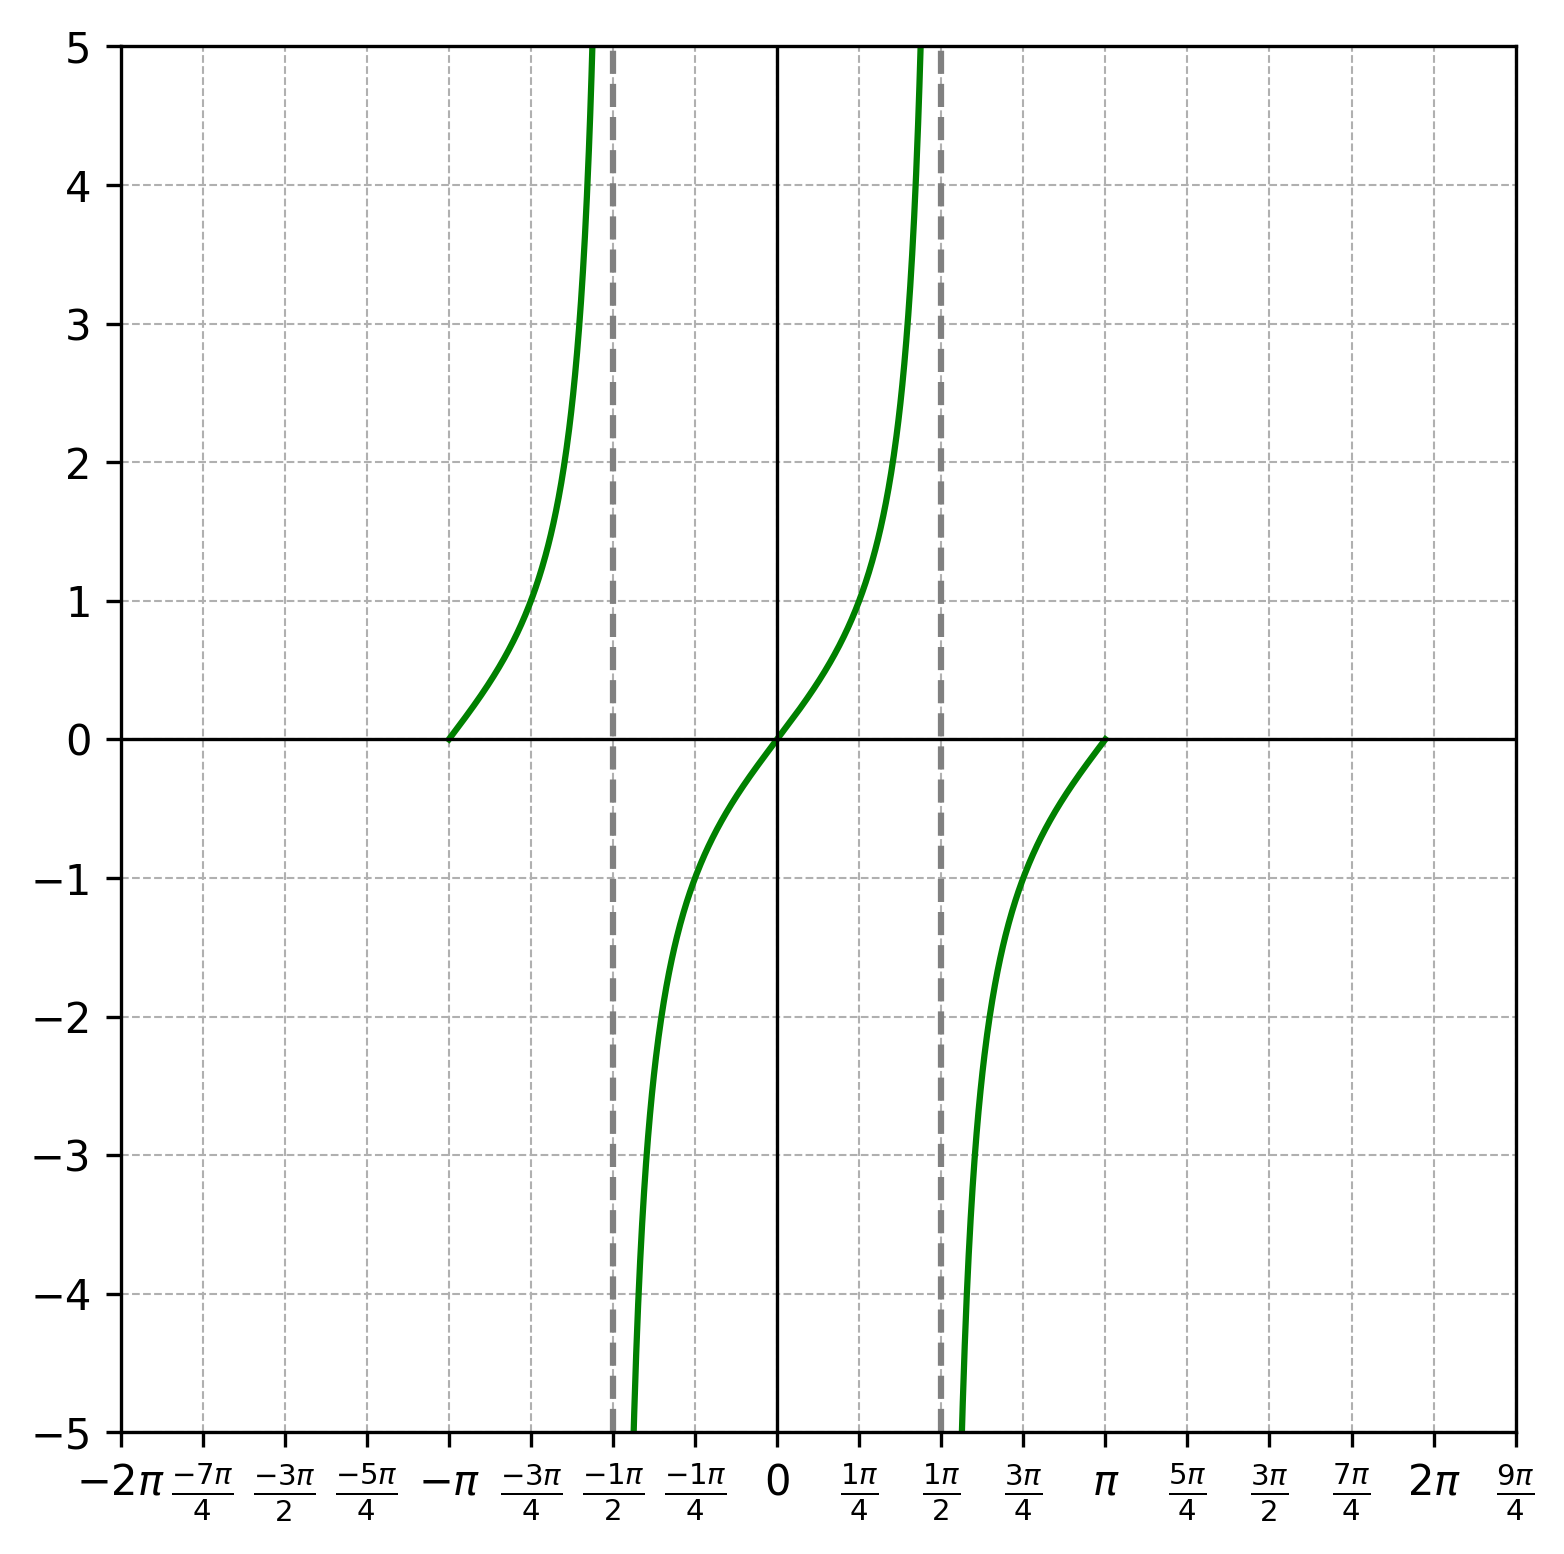
\includegraphics[width=0.5\textwidth]{./img/tangente.png}
    \caption{Grafico della funzione tangente con i suoi asintoti verticali.}
    \label{fig:tangente}
\end{figure}
\FloatBarrier

\subsubsection{Proprietà della Tangente}
\begin{itemize}
    \item \textbf{Periodicità:} È periodica con periodo \(T = \pi\).
    \item \textbf{Simmetrie:} È una funzione \textbf{dispari} (\(\tan(-x) = -\tan(x)\)).
\end{itemize}

\subsection{Funzioni Trigonometriche Inverse}
Per definire le funzioni inverse, è necessario restringere il dominio delle funzioni di partenza per renderle biettive.

\subsubsection{Arcoseno e Arcocoseno}
\begin{itemize}
    \item \textbf{Arcoseno (\(\arcsin\))}: È l'inversa della funzione seno ristretta a \(\left[-\frac{\pi}{2}, \frac{\pi}{2}\right]\).
    \[ \arcsin: [-1, 1] \rightarrow \left[-\frac{\pi}{2}, \frac{\pi}{2}\right] \]
    \item \textbf{Arcocoseno (\(\arccos\))}: È l'inversa della funzione coseno ristretta a \([0, \pi]\).
    \[ \arccos: [-1, 1] \rightarrow [0, \pi] \]
\end{itemize}

\begin{figure}[H]
    \centering
    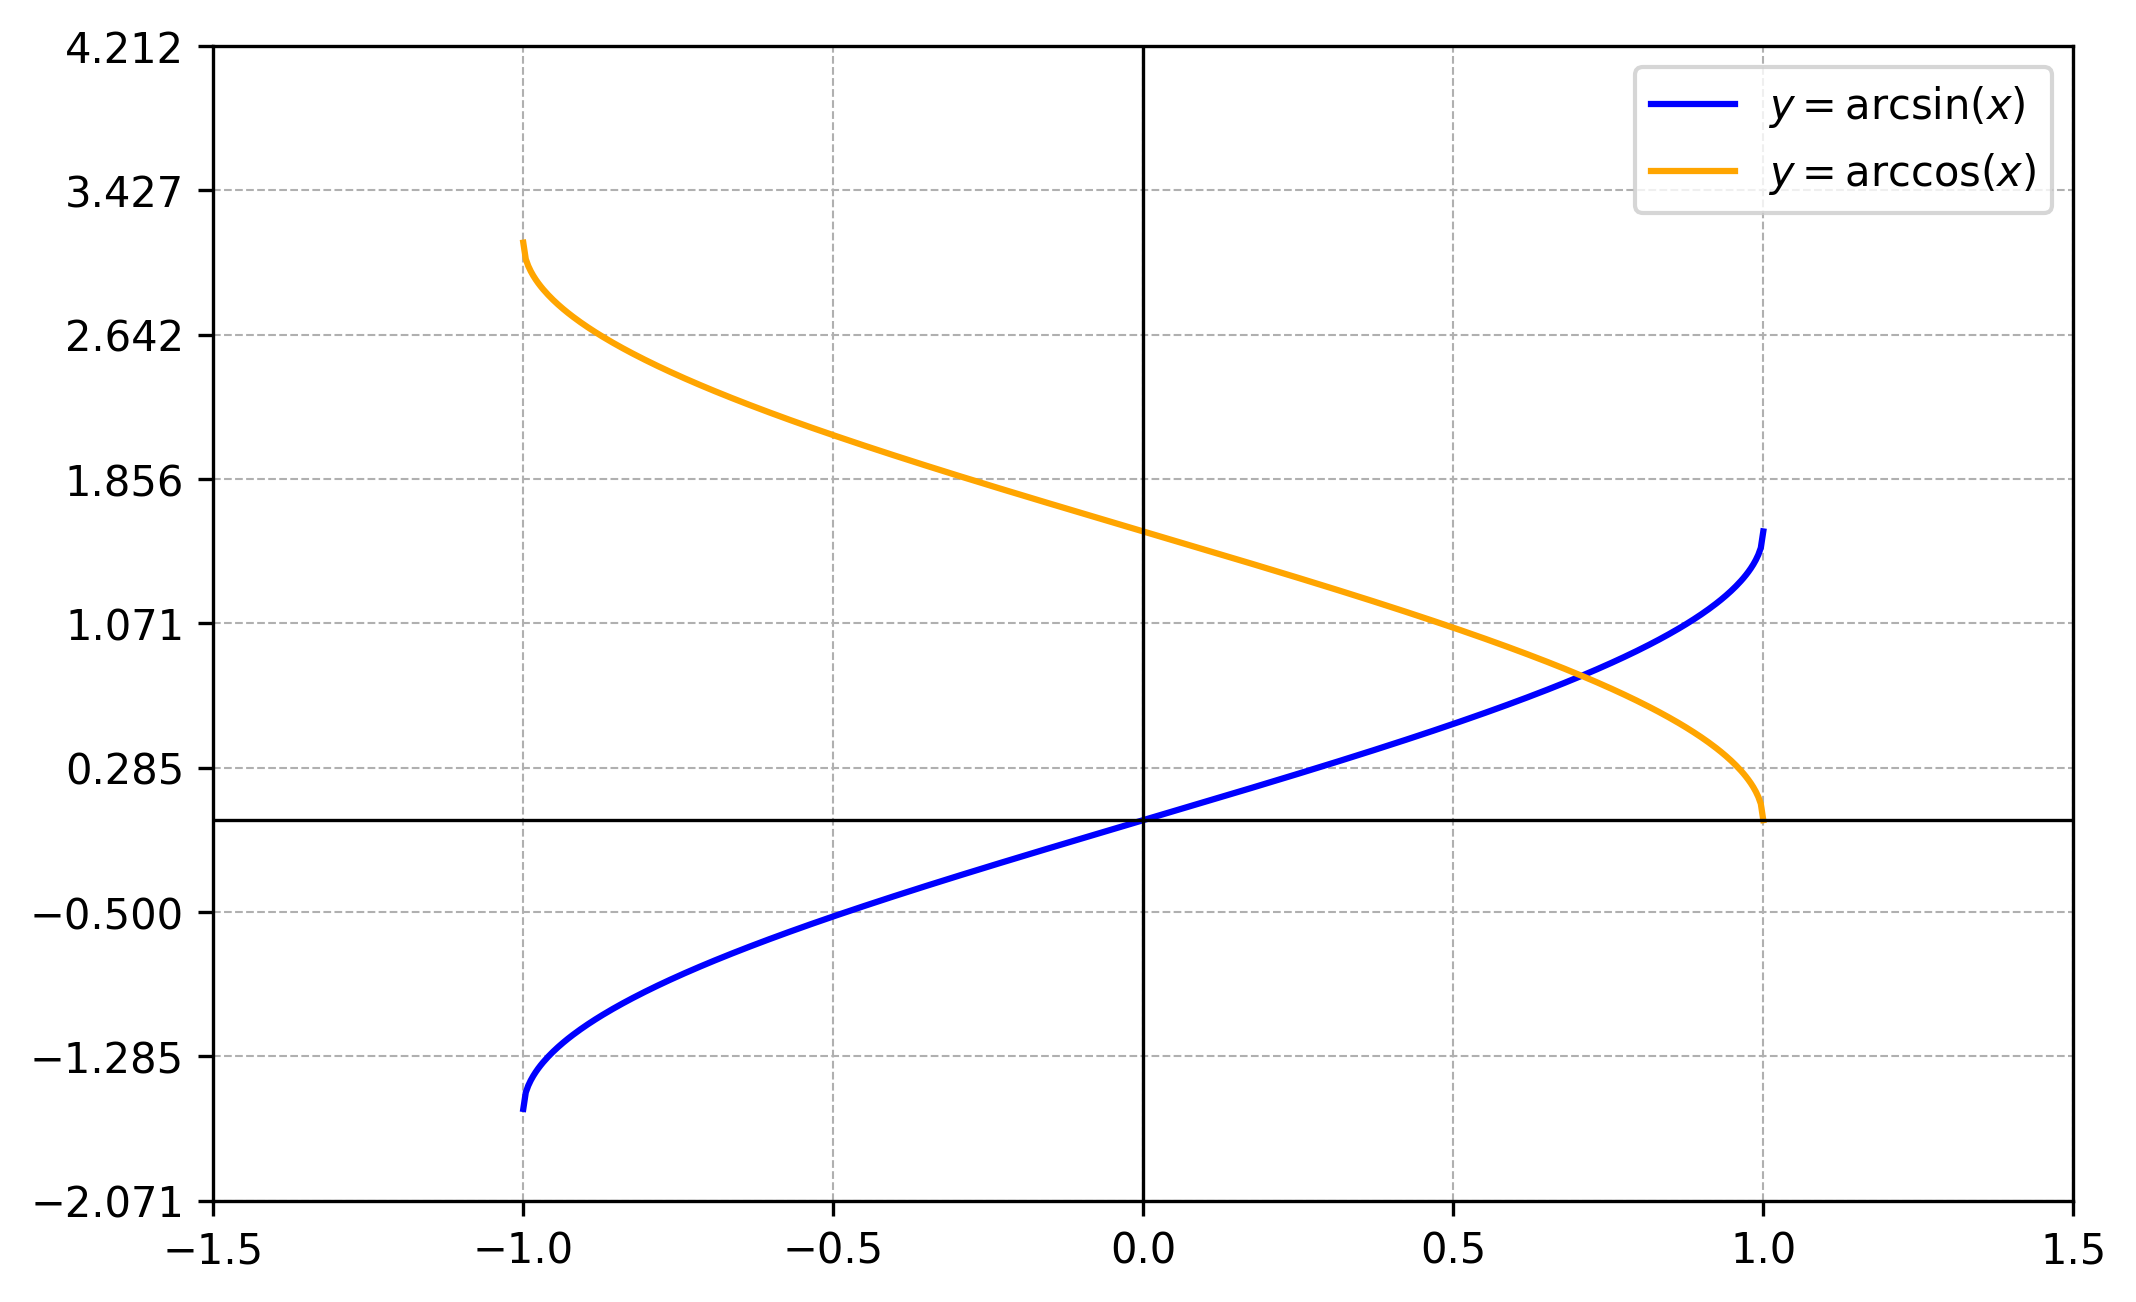
\includegraphics[width=0.8\textwidth]{./img/arcsin_arccos_grafici.png}
    \caption{Grafici delle funzioni \(y=\arcsin(x)\) (blu) e \(y=\arccos(x)\) (arancione).}
    \label{fig:arcsin_arccos_grafici}
\end{figure}
\FloatBarrier

\subsubsection{Arcotangente}
È l'inversa della funzione tangente ristretta a \(\left]-\frac{\pi}{2}, \frac{\pi}{2}\right[\).
\[ \arctan: \mathbb{R} \rightarrow \left]-\frac{\pi}{2}, \frac{\pi}{2}\right[ \]

\begin{figure}[H]
    \centering
    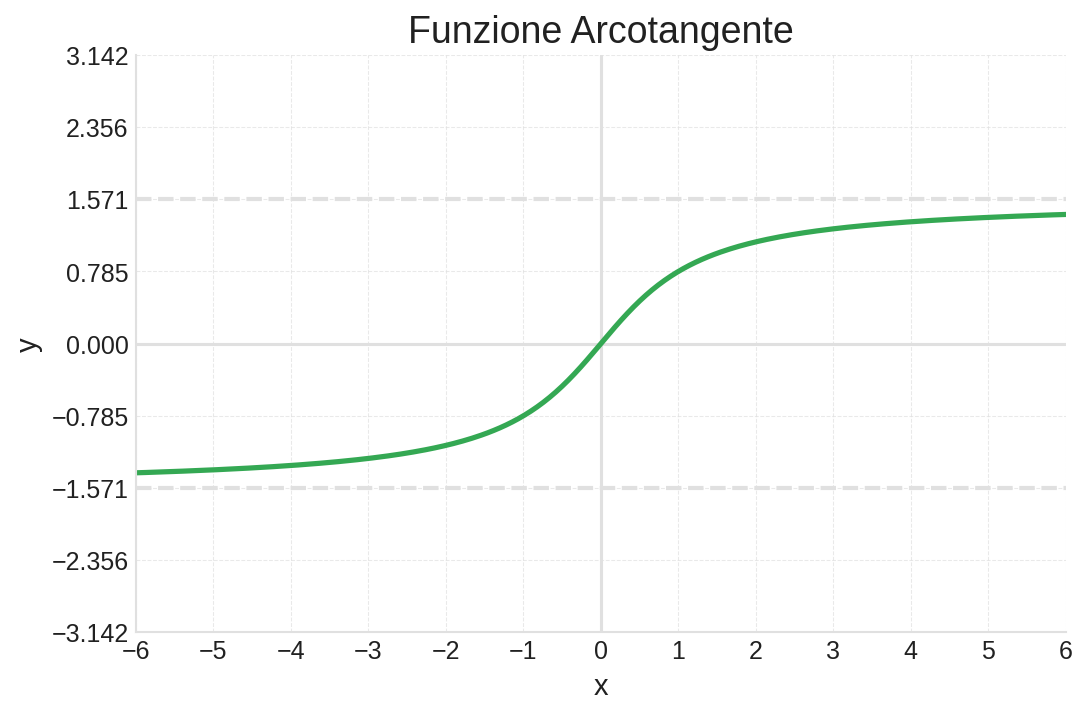
\includegraphics[width=0.6\textwidth]{./img/arcotangente.png}
    \caption{Grafico della funzione arcotangente con i suoi asintoti orizzontali.}
    \label{fig:arcotangente}
\end{figure}
\FloatBarrier

\subsection{Funzioni Iperboliche}
Definiamo il Seno Iperbolico ($\sinh x$) e il Coseno Iperbolico ($\cosh x$):

\begin{itemize}
    \item \textbf{Seno Iperbolico ($\sinh x$)} (Dispari):
    \[ \sinh x = \frac{e^x - e^{-x}}{2} \]
    Dominio: $\mathbb{R} \to \mathbb{R}$ [2].
    
    \begin{figure}[h]
        \centering
        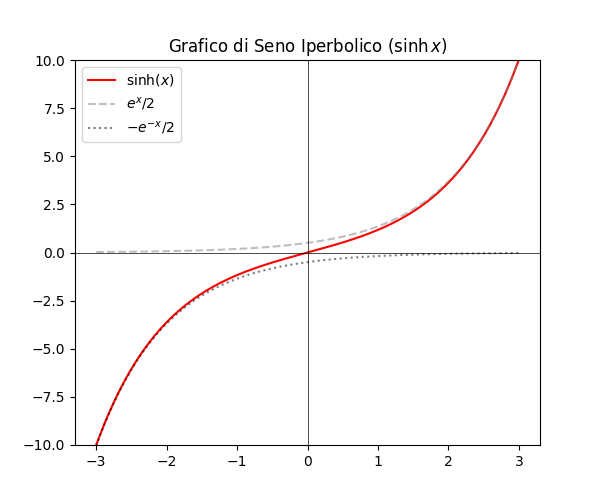
\includegraphics[width=0.45\textwidth]{img/grafico_senh.png} % Placeholder per grafico e^x, e^-x e sinh x
        \caption{Grafico di $\sinh x$ (come differenza tra $e^x/2$ e $-e^{-x}/2$). Cfr. [2]}
    \end{figure}

    \item \textbf{Coseno Iperbolico ($\cosh x$)} (Pari):
    \[ \cosh x = \frac{e^x + e^{-x}}{2} \]
    Dominio: $\mathbb{R} \to [1, +\infty[$.

    \begin{figure}[h]
        \centering
        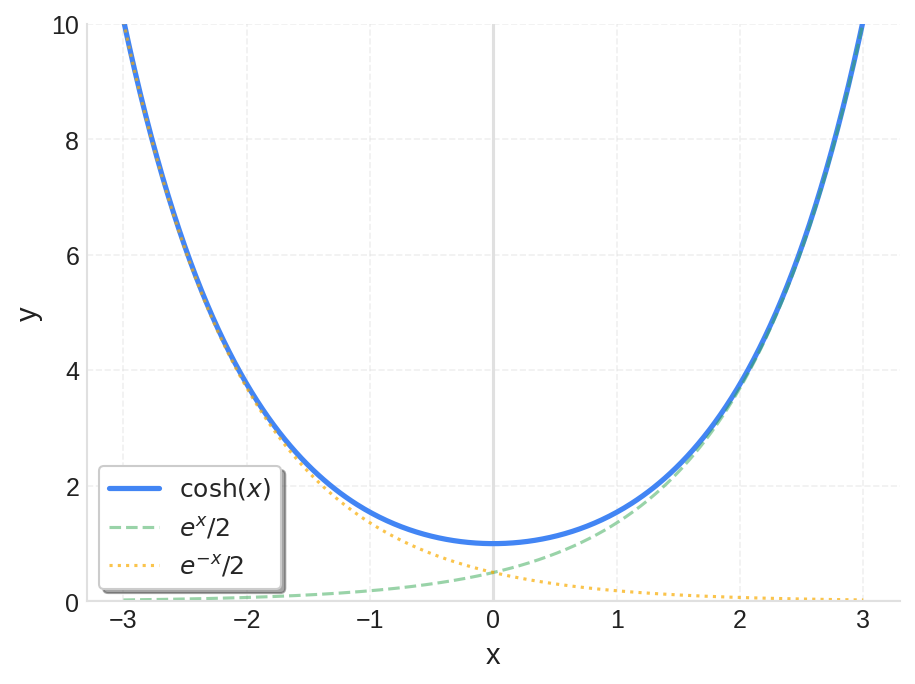
\includegraphics[width=0.45\textwidth]{img/grafico_cosh.png} % Placeholder per grafico e^x, e^-x e cosh x
        \caption{Grafico di $\cosh x$ (come somma di $e^x/2$ e $e^{-x}/2$). Cfr. [2]}
    \end{figure}
\end{itemize}
Le funzioni iperboliche sono connesse all'iperbole $x^2 - y^2 = 1$. L'inversa del seno iperbolico è $\operatorname{sett}\sinh x: \mathbb{R} \to \mathbb{R}$. L'inversa del coseno iperbolico è $\operatorname{sett}\cosh x: [1, +\infty[ \to [0, +\infty[$.


  Usiamo la stessa notazione delle funzioni trigonometriche perché $sinh$ e $cosh$ sono rispettivamente l'ascissa e l'ordinata di un punto $P$ che si sta muovendo su un ramo di iperbole.

\subsection{Trasformazioni del Grafico di Funzioni}
Le trasformazioni includono traslazioni verticali ($f(x) \pm K$), traslazioni orizzontali ($f(x \pm K)$), dilatazioni/contrazioni, e ribaltamenti.

\begin{itemize}
\item Traslazione verticale: $f_1(x) = f(x) \pm K$.
  \begin{figure}[H] % Usato [H] da float per forzare la posizione
    \centering
    % SOSTITUIRE 'img/traslazione_verticale.png' con il percorso del tuo file
    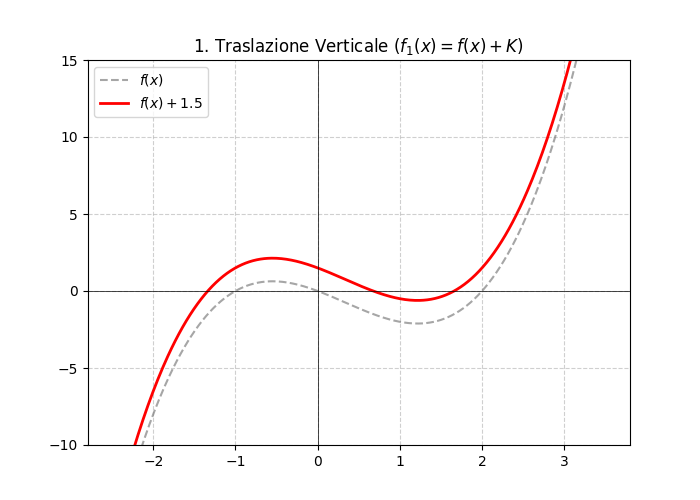
\includegraphics[width=0.45\textwidth]{img/traslazione_verticale.png}
    \caption{Traslazione verticale: $f(x)$ (grigio) e $f(x)+K$ (rosso).}
  \end{figure}

\item Traslazione orizzontale: $f_2(x) = f(x \pm K)$.
    \begin{figure}[H]
    \centering
    % SOSTITUIRE 'img/traslazione_orizzontale.png' con il percorso del tuo file
    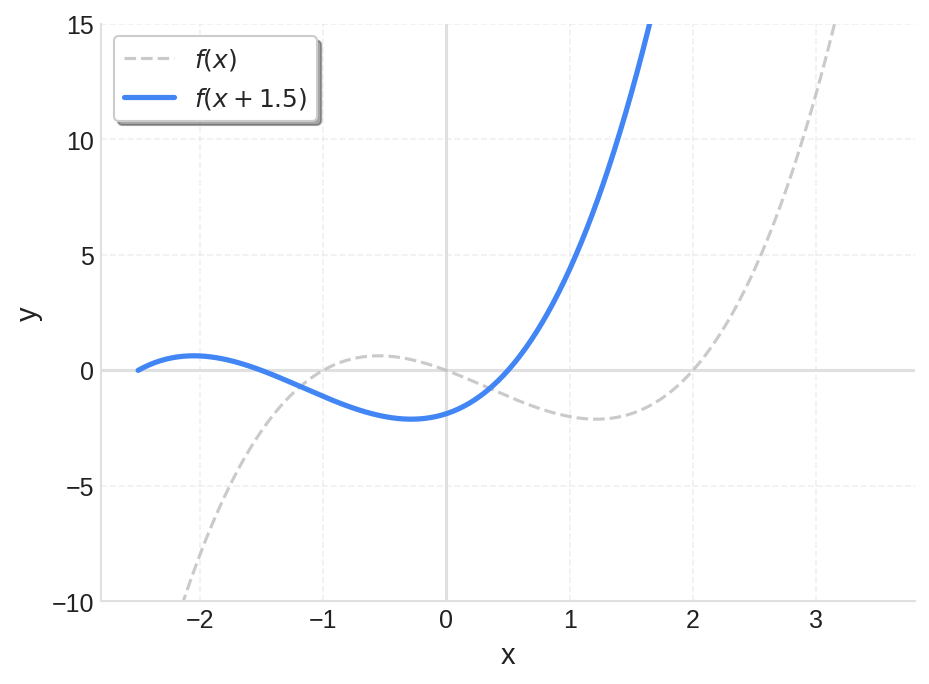
\includegraphics[width=0.45\textwidth]{img/traslazione_orizzontale.png}
    \caption{Traslazione orizzontale: $f(x)$ (grigio) e $f(x+K)$ (rosso).}
  \end{figure}

\item Dilatazione/Contrazione: $f_3(x) = K f(x)$ o $f(K x)$.
    \begin{figure}[H]
    \centering
    % NOTA: Questa immagine contiene due subplot (K f(x) e f(K x))
    % SOSTITUIRE 'img/dilatazione_contrazione.png' con il percorso del tuo file
    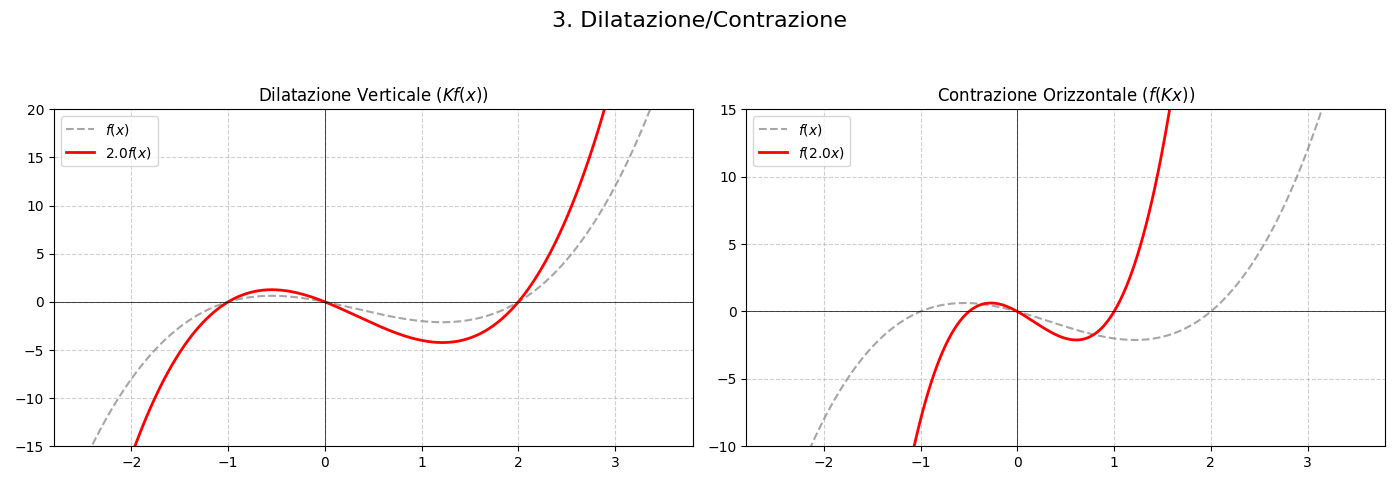
\includegraphics[width=0.9\textwidth]{img/dilatazione.png}
    \caption{Sinistra: Dilatazione verticale ($K f(x)$). Destra: Contrazione orizzontale ($f(K x)$).}
  \end{figure}

\item Ribaltamento rispetto all'asse $x$: $f_4(x) = -f(x)$.
    \begin{figure}[H]
    \centering
    % SOSTITUIRE 'img/ribaltamento_x.png' con il percorso del tuo file
    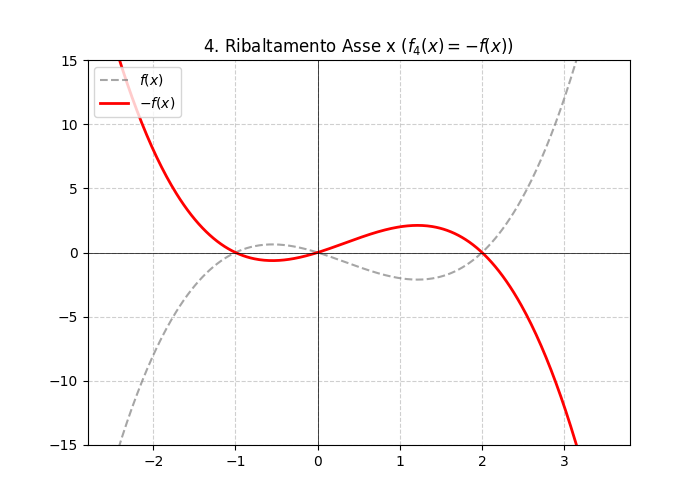
\includegraphics[width=0.45\textwidth]{img/ribaltamento_x.png}
    \caption{Ribaltamento asse x: $f(x)$ (grigio) e $-f(x)$ (rosso).}
  \end{figure}

\item Ribaltamento rispetto all'asse $y$: $f_5(x) = f(-x)$ (simmetria di specie).
    \begin{figure}[H]
    \centering
    % SOSTITUIRE 'img/ribaltamento_y.png' con il percorso del tuo file
    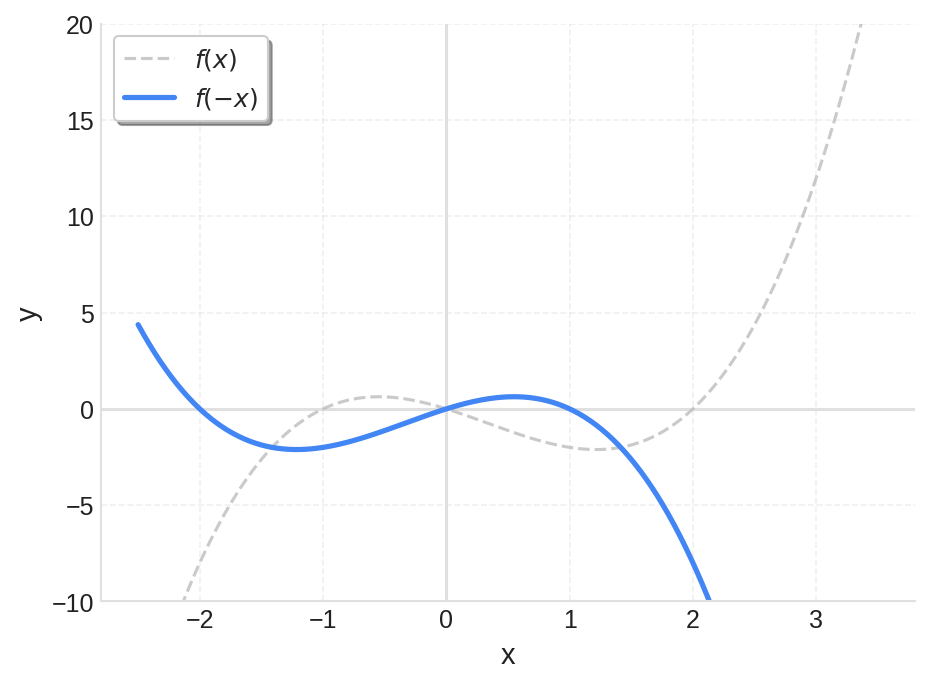
\includegraphics[width=0.45\textwidth]{img/ribaltamento_y.png}
    \caption{Ribaltamento asse y: $f(x)$ (grigio) e $f(-x)$ (rosso).}
  \end{figure}

\item Valore assoluto esterno: $f_6(x) = |f(x)|$.
    \begin{figure}[H]
    \centering
    % SOSTITUIRE 'img/valore_assoluto_esterno.png' con il percorso del tuo file
    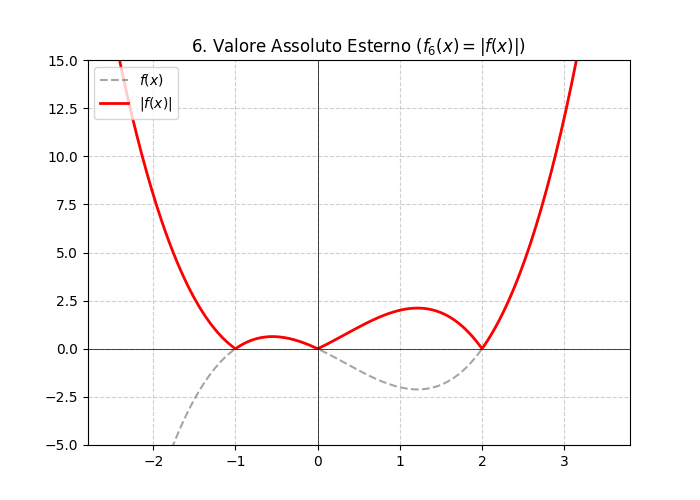
\includegraphics[width=0.45\textwidth]{img/valore_assoluto_esterno.png}
    \caption{Valore assoluto esterno: $f(x)$ (grigio) e $|f(x)|$ (rosso).}
  \end{figure}

\item Valore assoluto interno: $f_7(x) = f(|x|)$.
    \begin{figure}[H]
    \centering
    % SOSTITUIRE 'img/valore_assoluto_interno.png' con il percorso del tuo file
    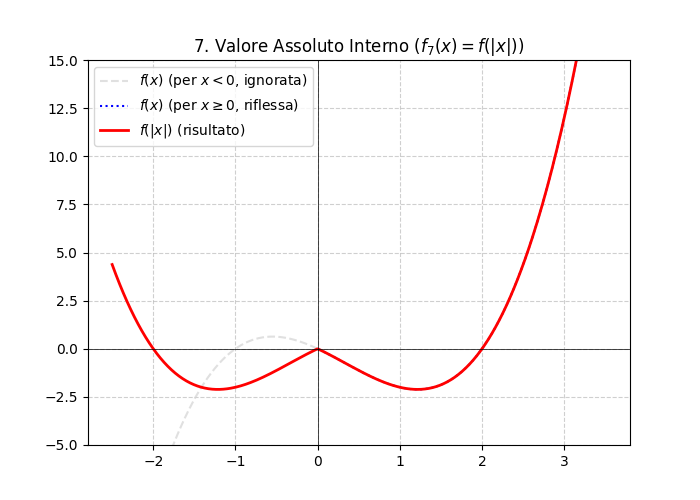
\includegraphics[width=0.45\textwidth]{img/valore_assoluto_interno.png}
    \caption{Valore assoluto interno: $f(x)$ (parti tratteggiate) e $f(|x|)$ (rosso).}
  \end{figure}
\end{itemize}